\documentclass{IEEEtran}
\usepackage{graphicx}
\usepackage{afterpage}
\usepackage{algorithm}
\usepackage{algpseudocode}
\usepackage{natbib}

\usepackage{url}

\title{Traffic Flow Prediction and Management}
\author{
    \IEEEauthorblockN{Arpan Verma (2022105), Aditya Upadhyay(2022040)}
    \newline
    \IEEEauthorblockN{
        Department of Computer Science Engineering\\
        INDRAPRASTHA INSTITUTE OF INFORMATION TECHNOLOGY\\
        New Delhi, INDIA\\
        Email: arpan22105@iiitd.ac.in, aditya22040@iiitd.ac.in
    }
}

\begin{document}

\maketitle

\begin{abstract}
Traffic congestion is a persistent challenge to urban mobility. Ineffective traffic flow causes commuters to spend time, use more fuel, and become frustrated.  This research explores state-of-the-art techniques and data-driven tactics in the field of traffic flow prediction and management.  We may proactively put solutions into place to reduce congestion, improve the timing of traffic lights, and improve the general effectiveness of transportation systems by anticipating future patterns in traffic. This paper looks at real-time management strategies, how machine learning improves traffic prediction, and how it might help cities become greener and more efficient in the future.
\end{abstract}

\section{Introduction}
Traffic congestion is a significant issue in urban areas, leading to wasted time, increased pollution, and economic losses. Effective traffic flow prediction and management are essential for alleviating congestion and improving transportation efficiency.
% \clearpage
\section{Stakeholders and there issues}
\textbf{Traffic congestion poses a significant challenge for a multitude of stakeholders
For local governments and transportation authorities, alleviating congestion is crucial for maintaining efficient transportation networks and ensuring economic vitality. Businesses depend on smooth traffic flow to facilitate the movement of goods and services, with delays potentially affecting productivity and delivery schedules. For residents, prolonged commute times and gridlock can lead to frustration, decreased quality of life, and even impacts on mental and physical health.

Addressing traffic flow is a crucial and holistic task that needs to be carried out efficiently and skilfully.
Thus for these reasons, such a Traffic flow Management System becomes even more important and a necessity.}
\begin{figure}[h]
    \centering
    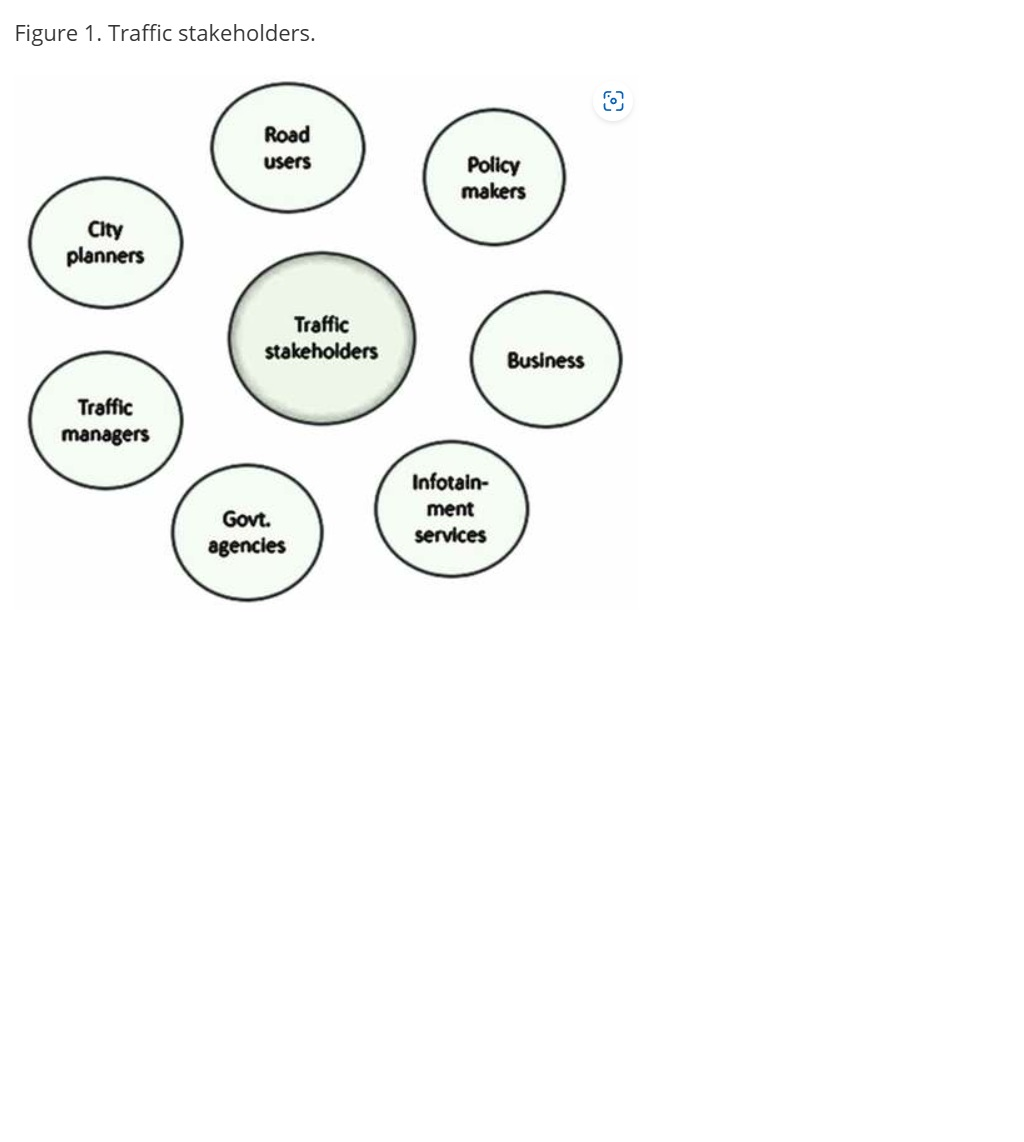
\includegraphics[width=0.8\textwidth]{displ3.jpg}
    
    \caption{Stakeholders}
    \label{fig:Stakeholders}
\end{figure}

\begin{figure}[h]
    \centering
    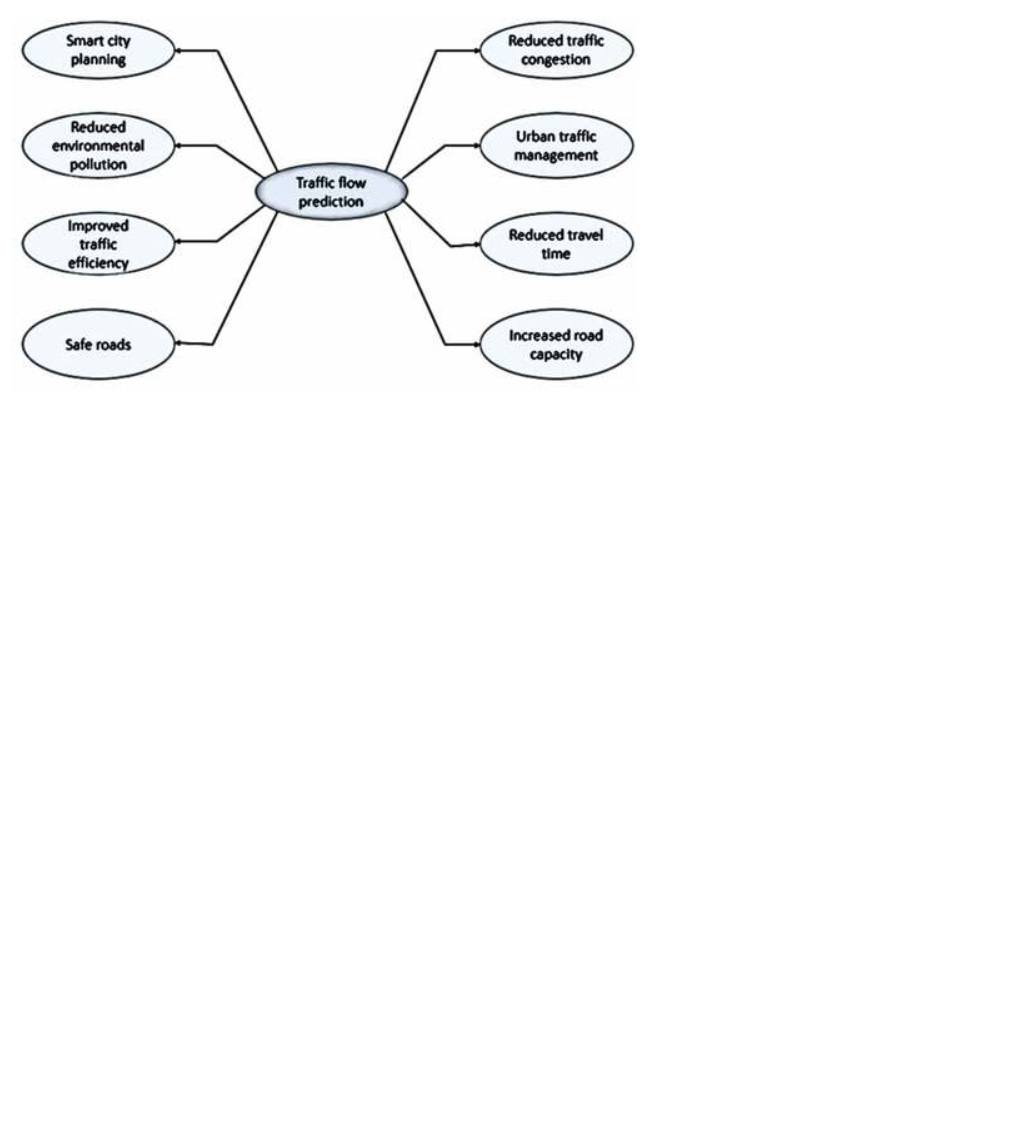
\includegraphics[width=0.8\textwidth]{displ.jpg}
    
    \caption{Model idea Usecases}
    \label{fig:Use cases}
\end{figure}
\begin{figure}[h]
    \centering
    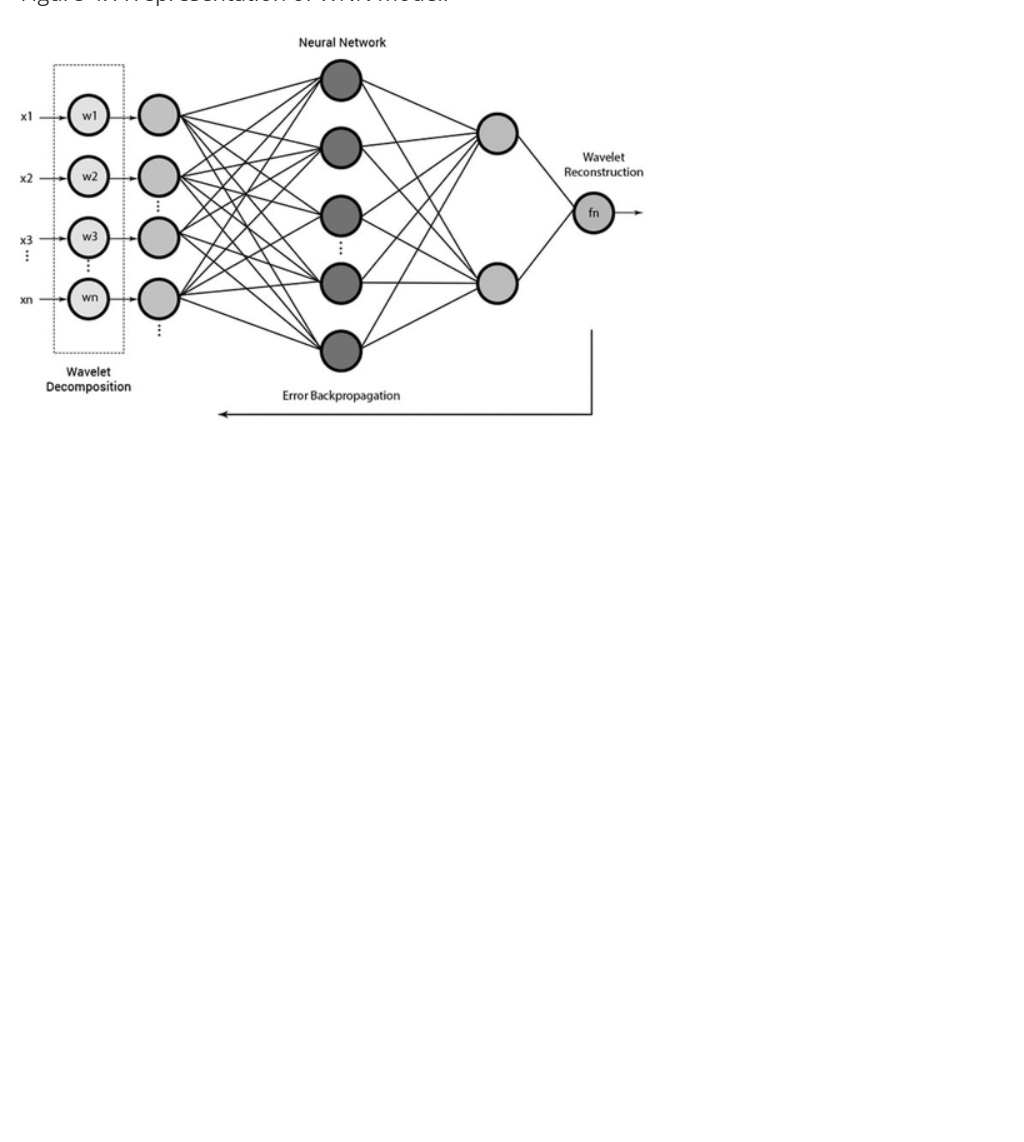
\includegraphics[width=0.8\textwidth]{displ2.jpg}
    
    \caption{Neural Network}
    \label{fig:Neural Network}
\end{figure}

\clearpage

\section{Methodology}
\subsection{Preprocessing}
For preprocessing of data we have done Normalization by subtracting Mean and dividing by square root of variance. There we also plotted for each feature available the corresponding elements this Step is done to visualize thse data samples there corresponding Need in Dataset.

\subsection{Model Used as First}
First we simply used Linear Regression as it is most simple to implement it is very useful in data where our training set is not much complex. This was just start try built from Scratch \newline
the equatation following for gradient descendent is : - 
\[
\frac{1}{n_{\text{samples}}} \cdot \text{np.dot}(X.T^\intercal, (y_{\text{pred}} - y))
\]
\newline
To reduce Mean square error Normalized the Function \newline
\text{df\_normalized} \leftarrow \frac{\text{df\_numerical} - \text{mean}(\text{df\_numerical})}{\text{std}(\text{df\_numerical})} \newline

\textbf{Here $df\_numerical$ are those columns that can be normalized.}

\textbf{Preprocessing: Handling NULL Values and feature extraction}

\text{data.fillna}(0)

\text{Explanation:} This step fills any missing values in the dataset with 0.

\textbf{Feature Engineering: Extract DateTime features}

\text{data['DateTime']} \leftarrow \text{pd.to_datetime(data['DateTime'])}

\text{data['Hour']} \leftarrow \text{data['DateTime'].dt.hour}

\text{data['DayOfWeek']} \leftarrow \text{data['DateTime'].dt.dayofweek}

\text{data['Month']} \leftarrow \text{data['DateTime'].dt.month}

\text{data['Year']} \leftarrow \text{data['DateTime'].dt.year}

\text{data["Date"]} \leftarrow \text{data['DateTime'].dt.day}

\text{Explanation:} These steps extract various date and time components from the 'DateTime' column and create new features such as hour, day of week, month, year, and date.

\textbf{Feature Engineering: Interaction Features}

\text{data['HourDayOfWeek']} \leftarrow \text{data['Hour']} \times \text{data['DayOfWeek']}

\text{Explanation:} This step creates an interaction feature by multiplying the hour and day of week features.

\textbf{Feature Engineering: Junction Features}

\text{data['Overall\_Traffic']} \leftarrow \text{data[['Junction\_1', 'Junction\_2', 'Junction\_3', 'Junction\_4']].sum(axis=1)}

\text{Explanation:} This step aggregates the traffic situation across all junctions to create a new feature representing overall traffic, which introduces some noise to prevent overfitting.

\textbf{Feature Engineering: Temporal Features}

\text{data['Trend']} \leftarrow \text{data.index}

\text{Explanation:} This step creates a trend feature based on the index of the data.

\textbf{Display the updated DataFrame with engineered features}

\subsection{Model 2 : Random Forest}
\text{The Random Forest Regressor model was trained and evaluated on two distinct datasets: one with normalized features and another with unnormalized features. This evaluation aimed to assess the impact of data normalization on model performance. The selected features for training and testing included 'Junction', 'Hour', 'DayOfWeek', and 'ID'. After fitting the regressor to the original training data, predictions were made on the corresponding test data for both normalized and unnormalized cases. Subsequently, mean squared error (MSE) was computed to quantify the prediction accuracy of the model.

Interestingly, the results revealed a notable improvement in model performance when utilizing normalized data. The MSE obtained from predictions made on the normalized dataset was considerably lower compared to the unnormalized counterpart. This observation underscores the significance of data preprocessing techniques, such as normalization, in enhancing the effectiveness of machine learning models.

Furthermore, the process involved experimentation with different parameter combinations to optimize model performance. By systematically evaluating various parameter settings, including the number of trees in the random forest and the maximum depth of each tree, the configuration yielding the lowest MSE and the best fit in y\_pred was identified. This rigorous parameter tuning process ensured that the model was fine-tuned to capture the underlying patterns in the data and produce accurate predictions.

To illustrate the impact of normalization and showcase the performance improvement achieved, a graphical representation of the MSE comparison between the normalized and unnormalized cases was generated. This visualization provided a clear depiction of the benefits conferred by data normalization, further reinforcing its importance in machine learning workflows.

In summary, the Random Forest Regressor exhibited promising performance in predicting the target variable. Through meticulous experimentation, parameter optimization, and data preprocessing, the model was effectively trained to accurately capture the relationships between the input features and the target variable, thereby demonstrating its suitability for the task at hand.}


\section{Comparison of Traffic Flow Prediction and Management Approaches}

This section compares different approaches to traffic flow prediction and management, evaluating their effectiveness and applicability in various scenarios.
\subsection{Model Comparison Linear}

We experimented with several models to predict traffic flow and manage traffic effectively. One of the models we tested was the Linear Regressor, which we implemented ourselves. However, this model performed poorly, especially considering the complexity of the dataset. 

\subsection{Gradient Boosting}

After observing the poor performance of the Linear Regressor, we explored Gradient Boosting as an alternative approach. While the findings were marginally better than those of the Linear Regressor, they still fell short of our expectations. We realized that the Linear Regressor struggled to separate the dataset into distinct parts by a straight line, leading us to shift our focus towards another regressor algorithm.

\subsection{Random Forest}

Random Forest emerged as a promising solution, providing satisfactory predictions for traffic flow. However, achieving these results required careful parameter tuning. We systematically tested various combinations of features to optimize model performance. Notably, the inclusion of 'Junction' and 'ID' features significantly improved prediction accuracy.

Upon closer examination, we discovered that the 'ID' feature played a crucial role in predicting traffic congestion. By analyzing the dataset, we observed that the 'ID' column contained dates and binary digits appended as numbers. Leveraging this insight, the model effectively predicted congestion patterns based on specific days. Disregarding the 'ID' feature resulted in inferior predictions, highlighting its importance in the modeling process.

While Random Forest successfully detected and predicted traffic congestion, there remains room for improvement. Despite its effectiveness, further enhancements are needed to address certain limitations and refine the model's performance.

\subsection{Gradient Boosting}
The Gradient Boosting Regressor algorithm, a powerful ensemble learning technique, is employed to build the regression model. This model is trained on the training data and subsequently used to make predictions on the testing data. The mean squared error (MSE) metric is calculated to assess the model's performance, representing the average squared difference between the predicted and actual number of vehicles. The goal of this code is to minimize the MSE, indicative of better predictive accuracy. By iteratively adjusting model hyperparameters, conducting feature engineering, and evaluating various algorithms, the aim is to refine the model and ultimately enhance its predictive capabilities for traffic flow prediction.

% Additional subsections and details can be added as required



\section{Findings}

\subsection{Traffic Flow Prediction Results}
\textbf{We found Data Follows some Trend like on holidays Vehicle count generally increases. We can see this growth and it is quite supportive in a way that on holidays Generally increases}

\subsection{Data Visualization and Junction Pie Chart}

Despite efforts to gain insights into traffic patterns through data visualization, the results did not reveal significant trends or patterns. Figure \ref{fig:data_visualization} shows the visualization of traffic distribution across different junctions, which unfortunately did not yield actionable insights. Similarly, Figure \ref{fig:junction_pie_chart} presents the percentage distribution of traffic among junctions using a pie chart, with no discernible patterns or trends observed.

\begin{figure}[h]
    \centering
    \begin{subfigure}{0.48\textwidth}
        \centering
        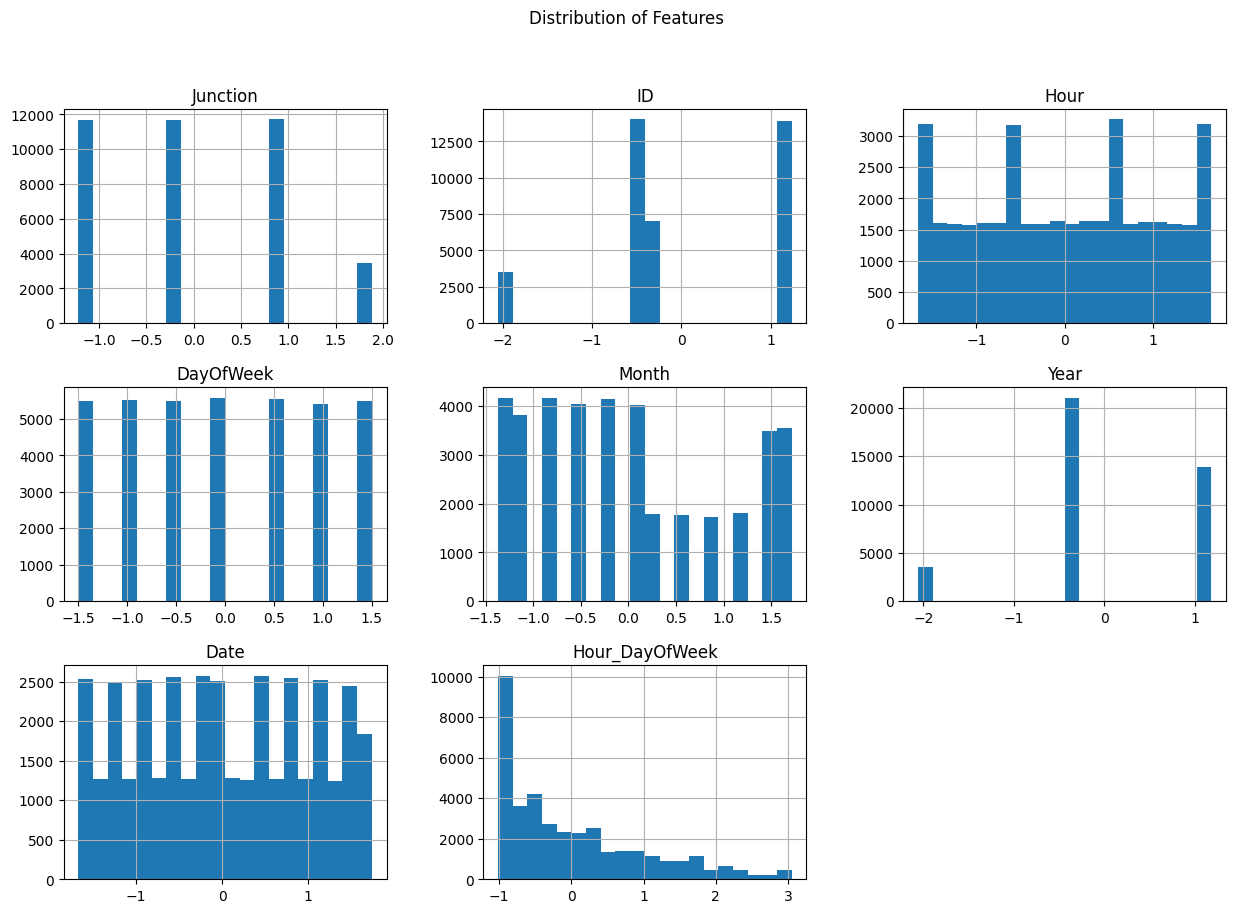
\includegraphics[width=10cm, height=6cm]{data_visualisation.png}
        \caption{Traffic distribution across junctions.}
        \label{fig:data_visualization}
    \end{subfigure}
    \hfill
    \begin{subfigure}{0.48\textwidth}
        \centering
        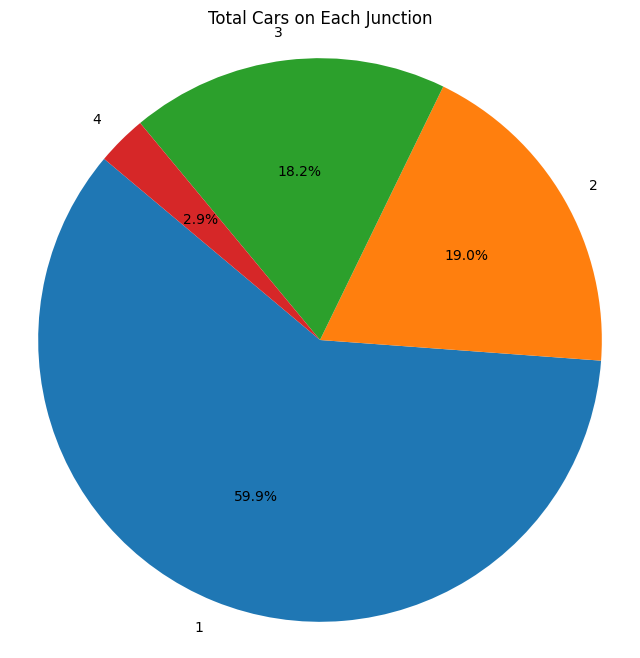
\includegraphics[width=10cm, height=6cm]{pie_chart.png}
        \caption{Percentage distribution of traffic across junctions.}
        \label{fig:junction_pie_chart}
    \end{subfigure}
    \caption{Inconclusive findings from data visualization and junction pie chart.}
\end{figure}
\clearpage

\subsection{How to select Features}
\begin{figure}[h]
    \centering
    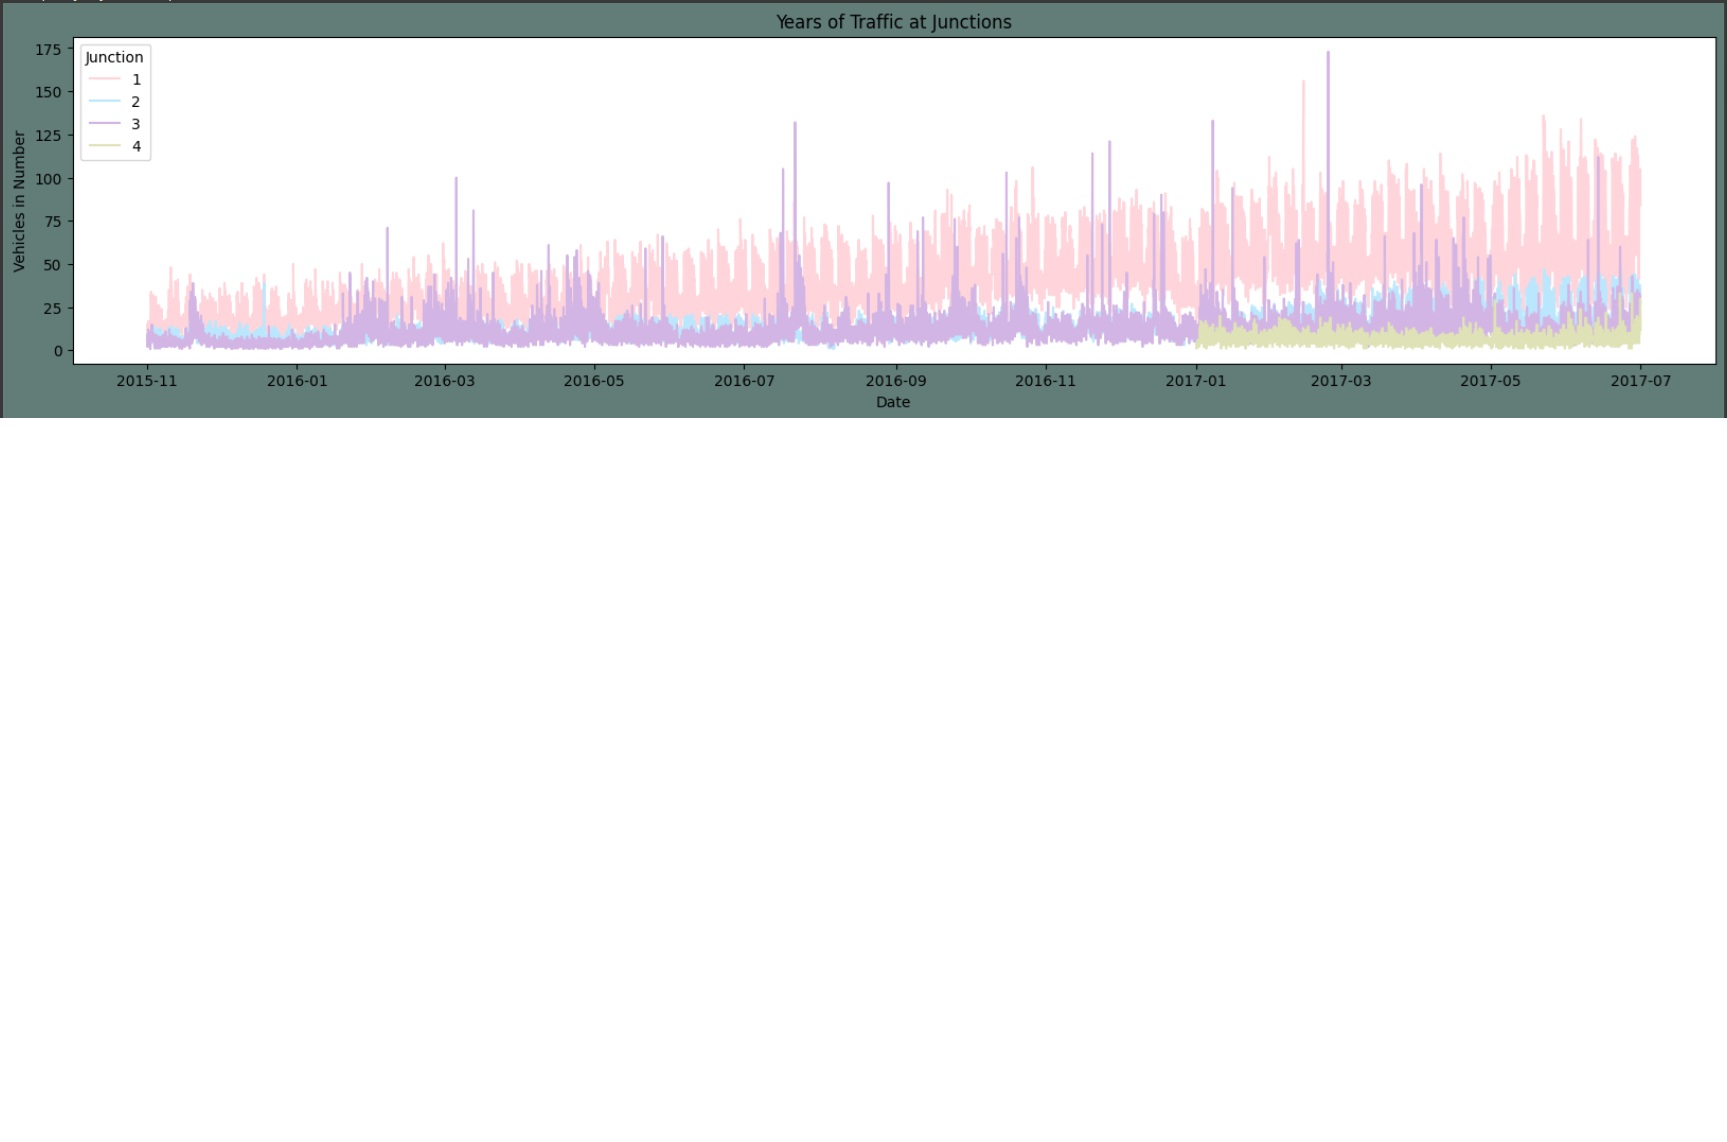
\includegraphics[width=0.8\textwidth]{JunctionvsDatetrend.jpg}
    
    \caption{Junction vehicles trend.}
    \label{fig:FeaturesSelectionHelper}
\end{figure}
\begin{figure}[h]
    \centering
    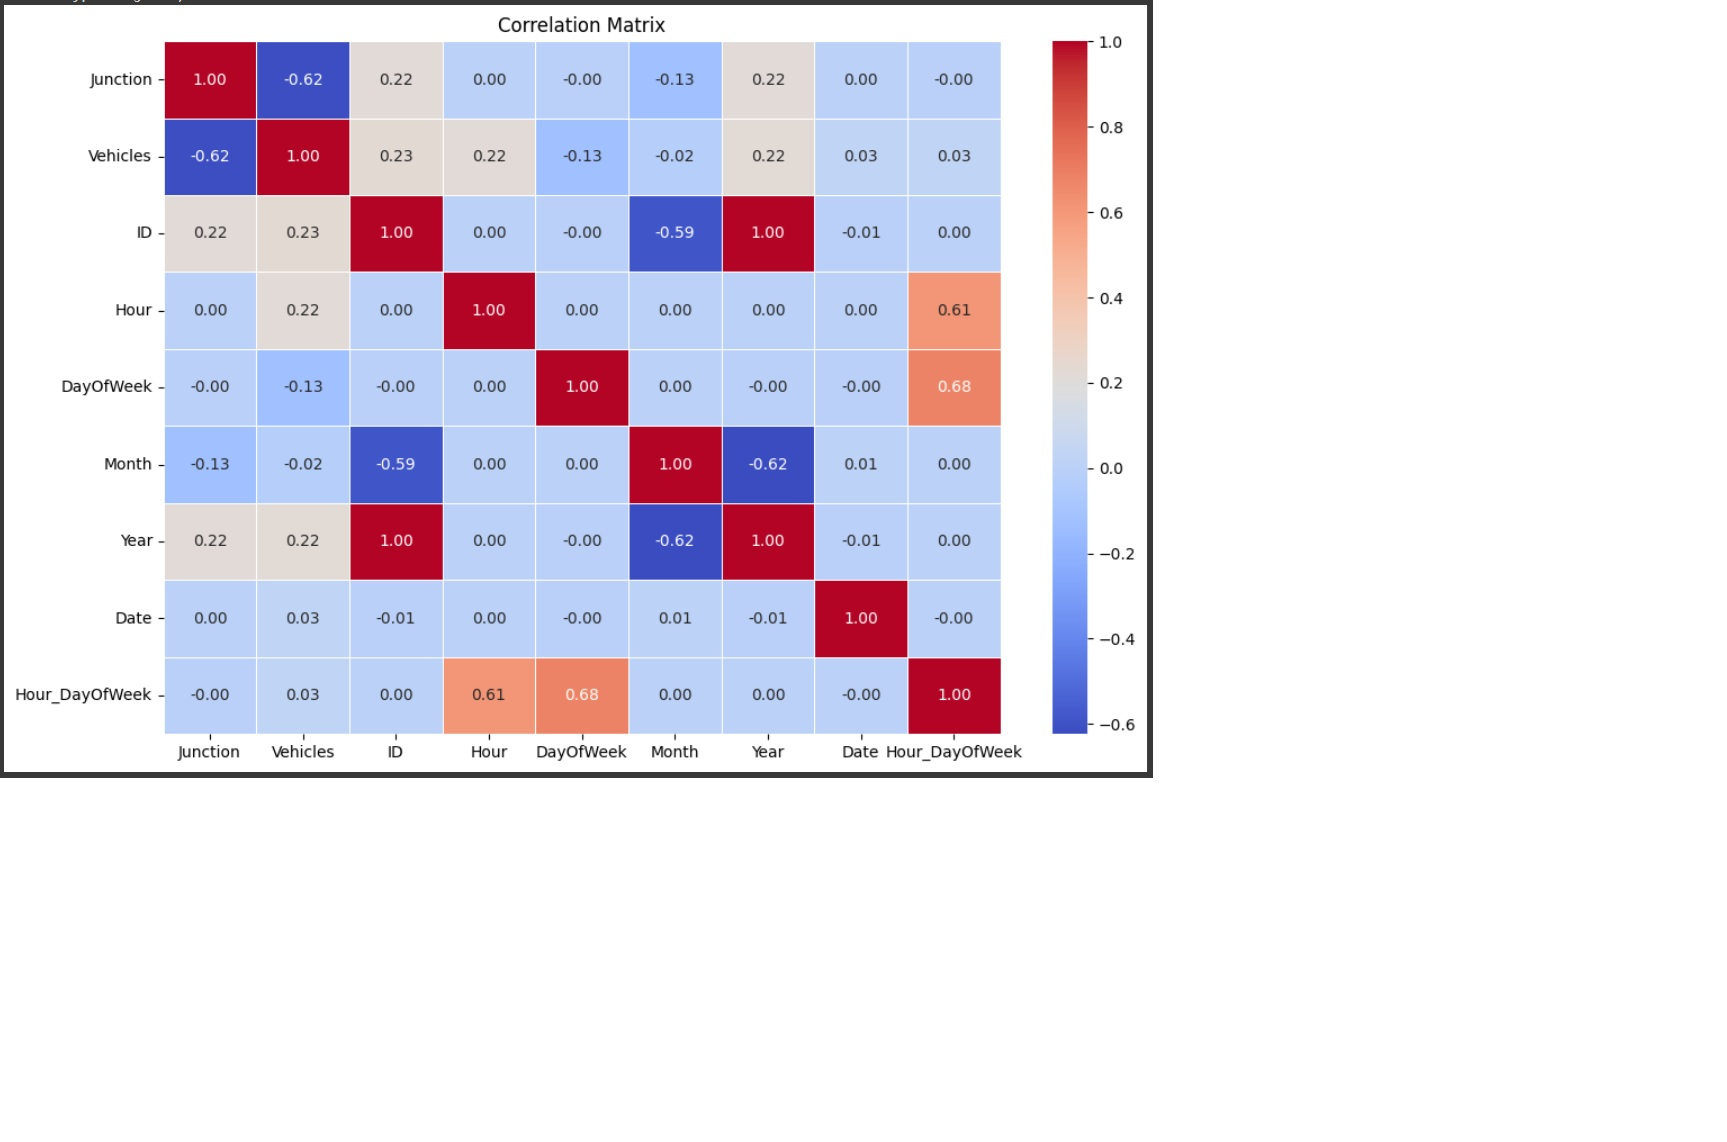
\includegraphics[width=0.8\textwidth]{Covariane_matrix.jpg}
    
    \caption{Covariance Matrix.}
    \label{fig:FeaturesSelectionHelper}
\end{figure}


% \clearpage

\textbf{We cannot select all the features; hence, we need to select the best. This can be done using the absolute correlation between features to select the features in corresponding vehicles.}
\clearpage
\subsection{Random Forest Regression Results}

The evaluation of the Random Forest Regression model yielded mixed results. Figure \ref{fig:random_forest_results} presents the prediction results obtained using the Random Forest Regression model.

\begin{figure}[p]
    \centering
    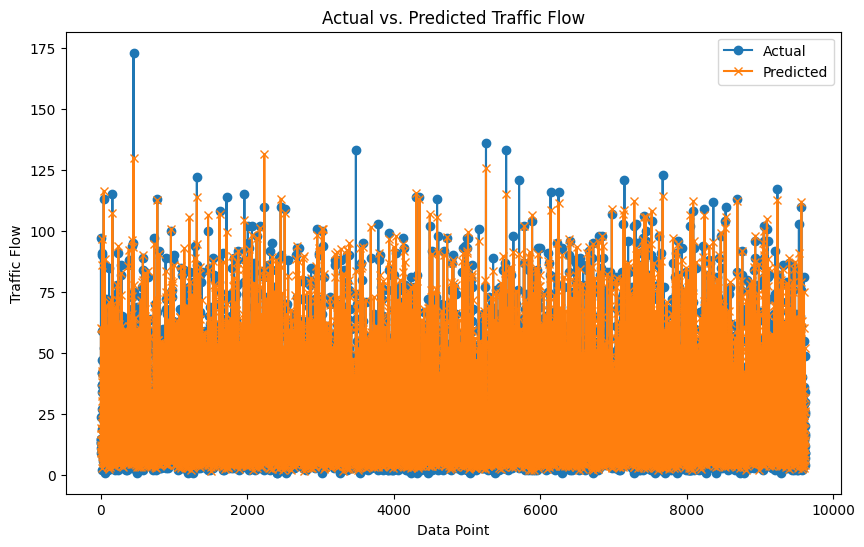
\includegraphics[width=10cm, height=10cm]{random_forest.png}
    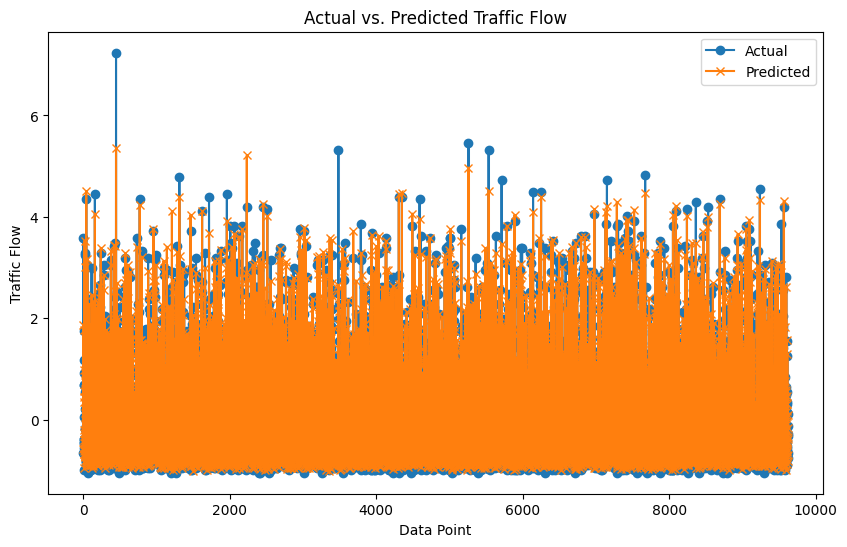
\includegraphics[width=10cm, height=10cm]{random_forest_norm.png}
    \caption{Traffic flow prediction results using Random Forest Regression model.}
    \label{fig:random_forest_results}
\end{figure}

\begin{figure}[p]
    \centering
    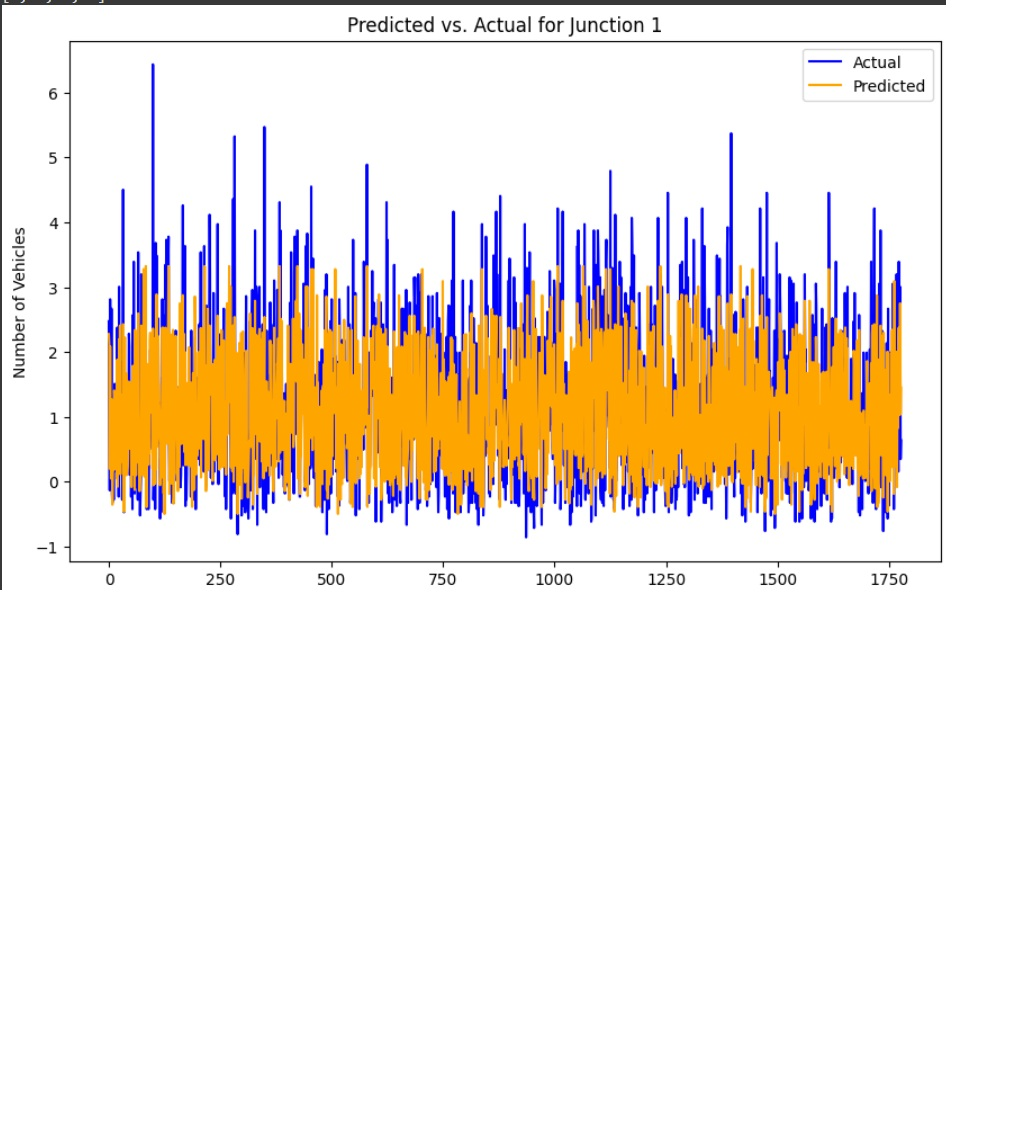
\includegraphics[width=7cm, height=8cm]{Random_forest_junc1.jpg}
    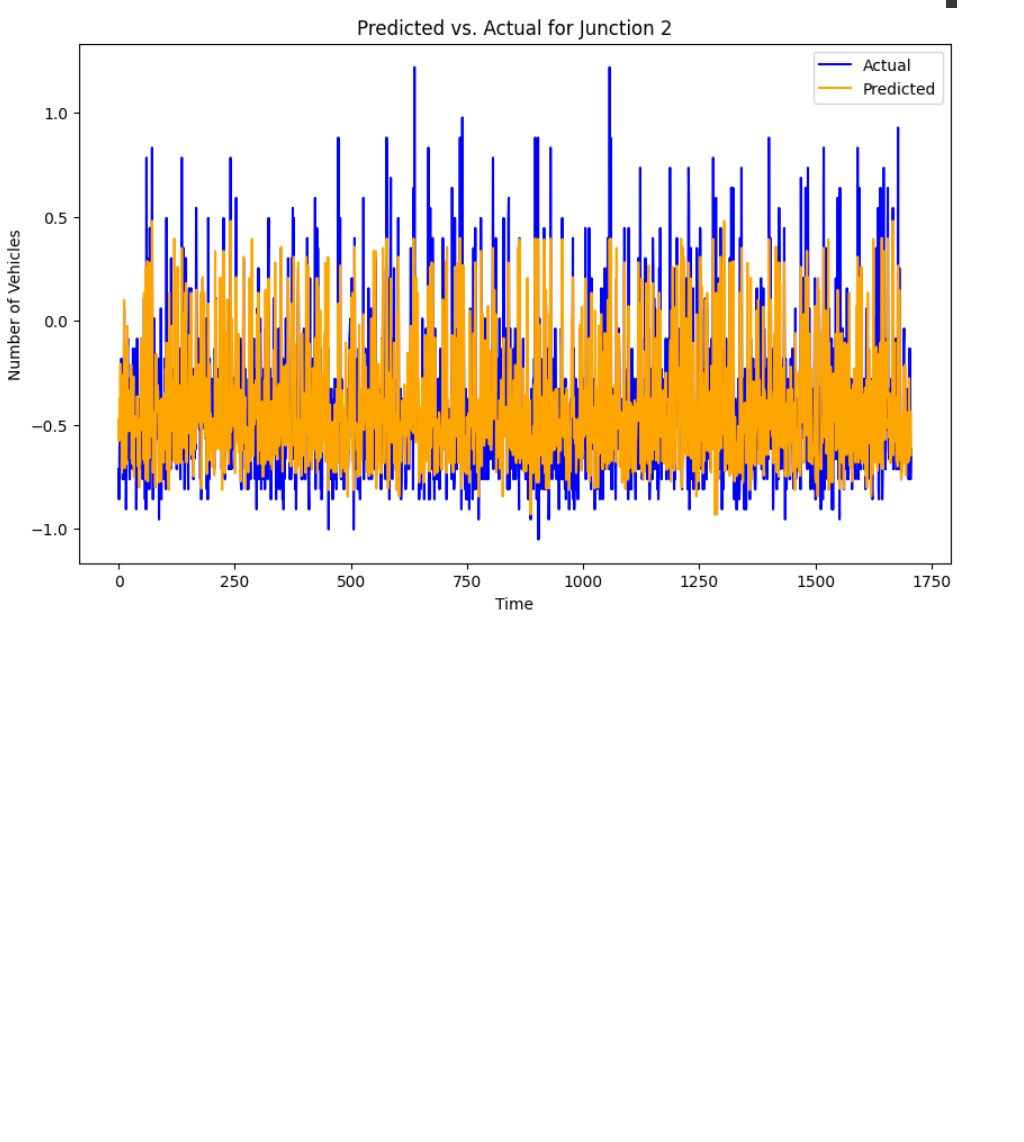
\includegraphics[width=7cm, height=8cm]{Random_forest_junc2.jpg}
    \caption{Random Forest Results for Junction 1 (left) and Junction 2 (right).}
    \label{fig:random_forest_junc_results}
\end{figure}

\begin{figure}[p]
    \centering
    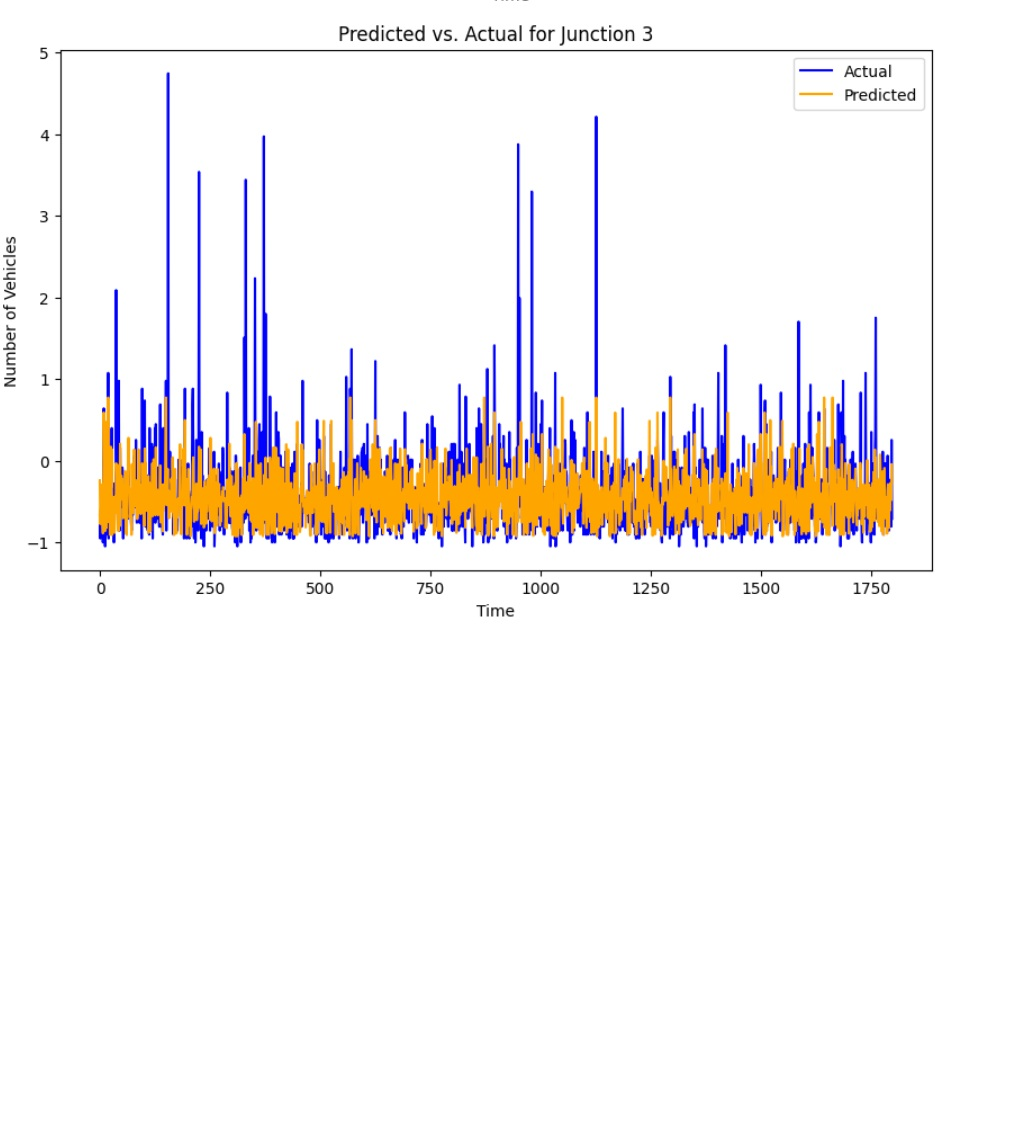
\includegraphics[width=7cm, height=8cm]{Random_forest_junc3.jpg}
    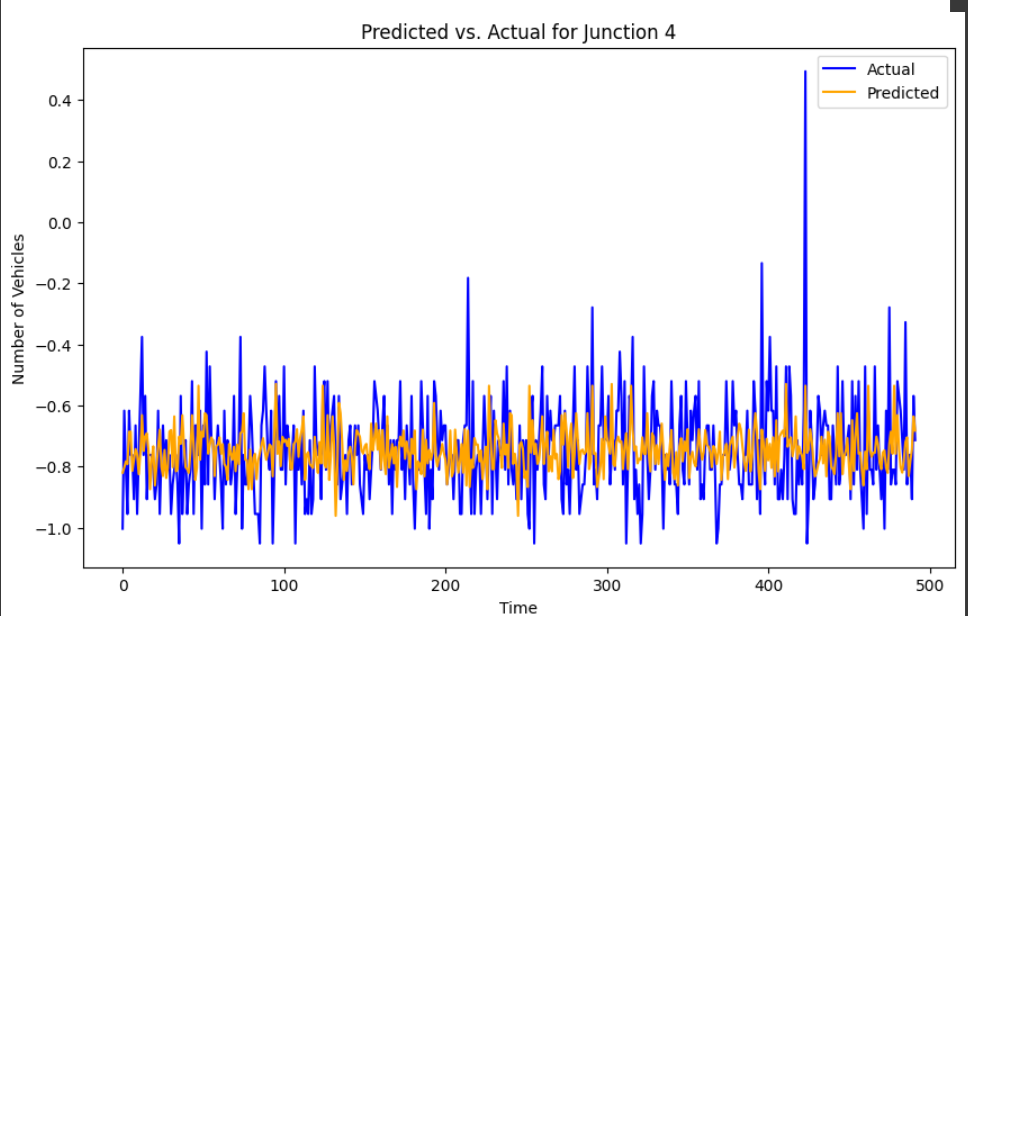
\includegraphics[width=7cm, height=8cm]{Random_forest_junc4.jpg}
    \caption{Random Forest Results for Junction 3 (left) and Junction 4 (right).}
    \label{fig:random_forest_junc_results2}
\end{figure}

% \begin{figure}[htbp]
%     \centering
%     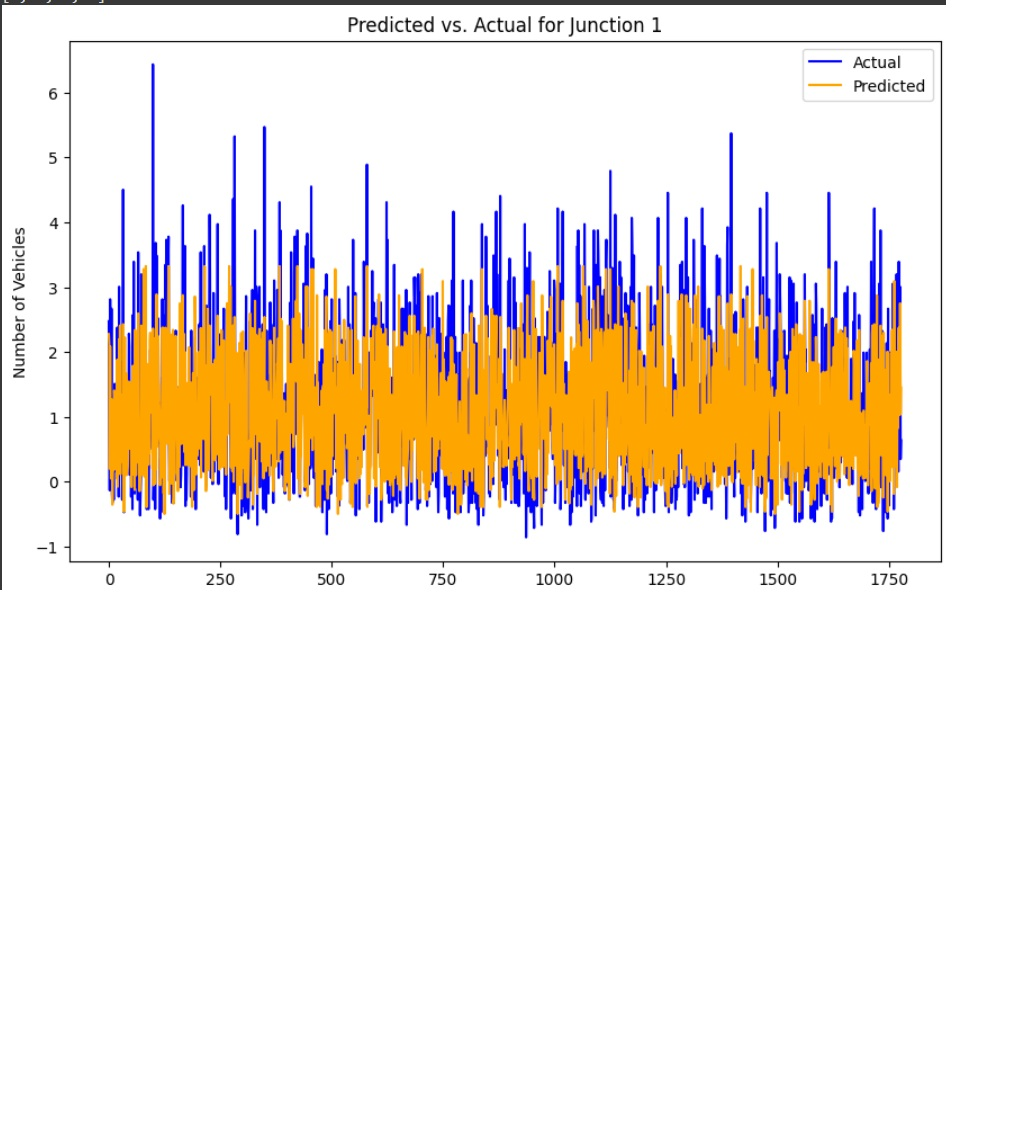
\includegraphics[width=0.8\textwidth]{Random_forest_junc1.jpg}
%     \caption{Random Forest Results for Junction 1}
%     \label{fig:random_forest_results_junction}
% \end{figure}
% \begin{figure}[htbp]
%     \centering
%     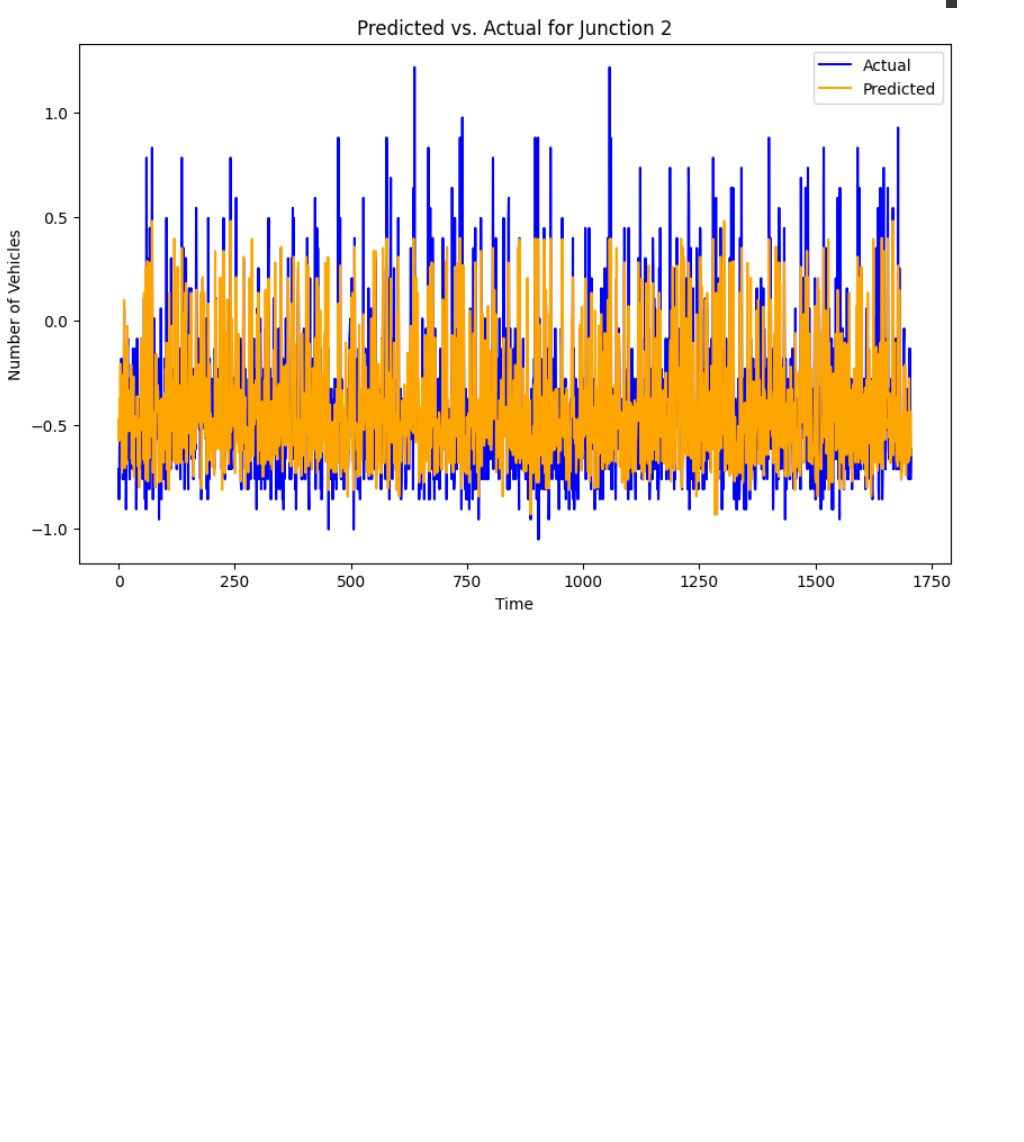
\includegraphics[width=0.8\textwidth]{Random_forest_junc2.jpg}
%     \caption{Random Forest Results for Junction 2}
%     \label{fig:random_forest_results_junction}
% \end{figure}
% \begin{figure}[htbp]
%     \centering
%     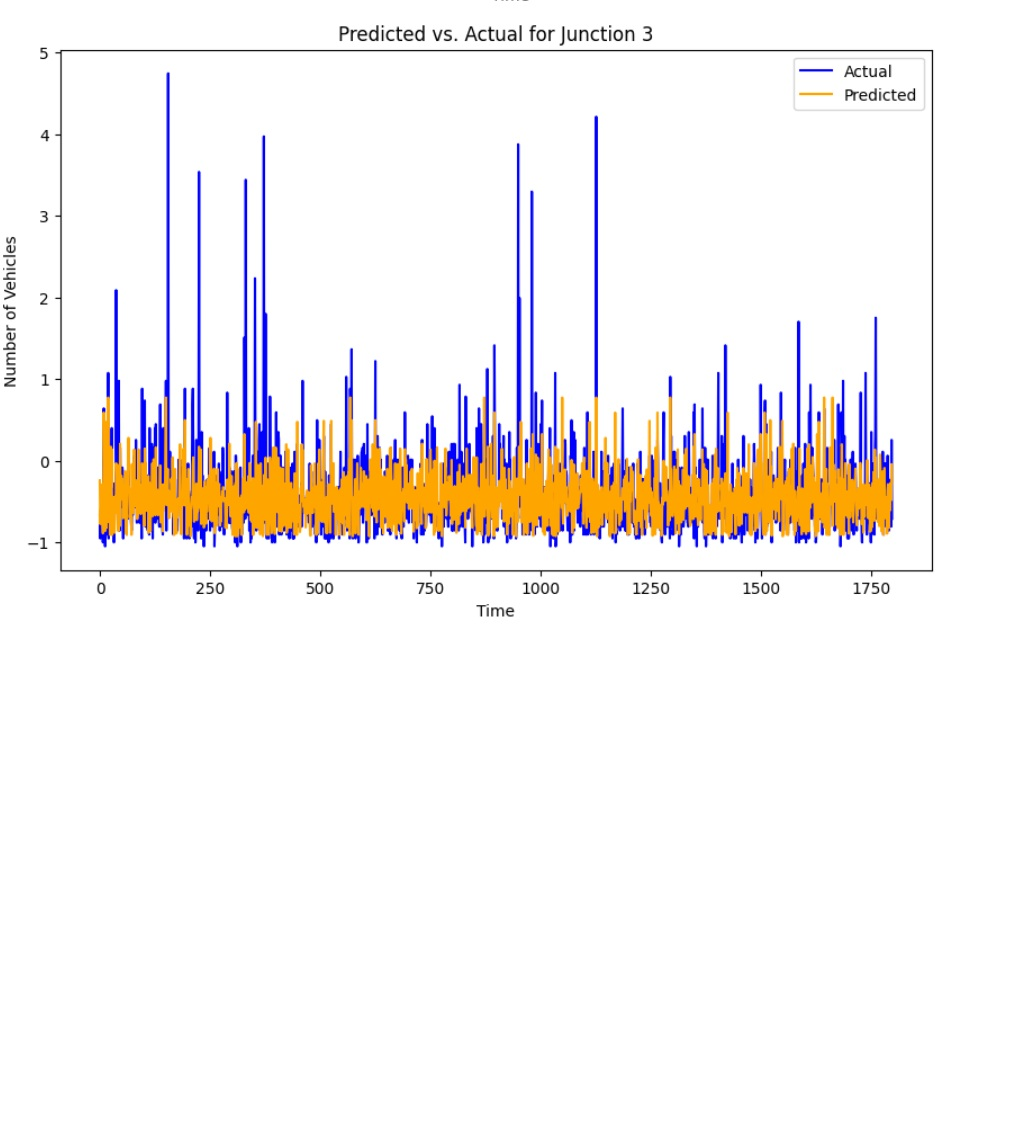
\includegraphics[width=0.8\textwidth]{Random_forest_junc3.jpg}
%     \caption{Random Forest Results for Junction 3}
%     \label{fig:random_forest_results_junction}
% \end{figure}
% \begin{figure}[htbp]
%     \centering
%     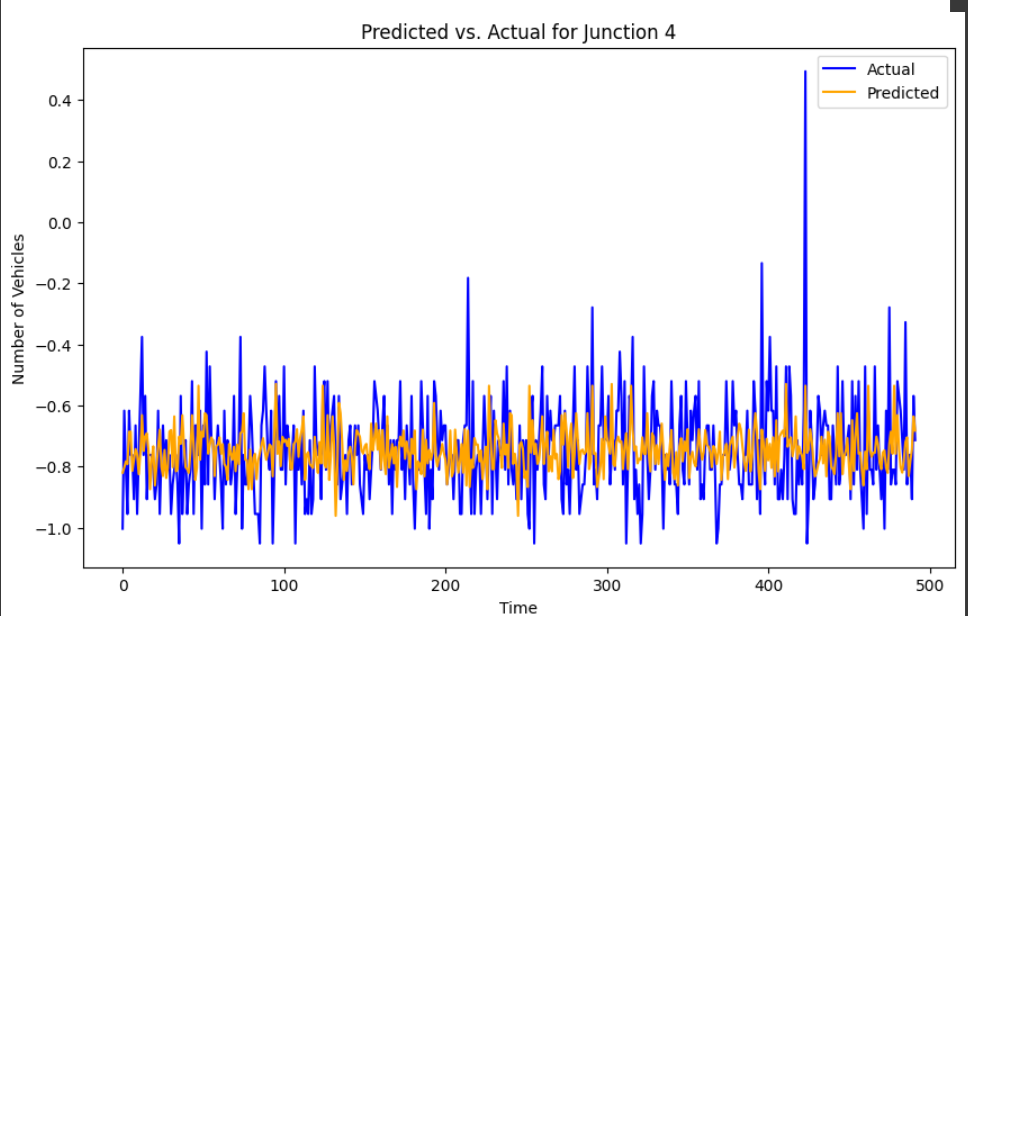
\includegraphics[width=0.8\textwidth]{Random_forest_junc4.jpg}
%     \caption{Random Forest Results for Junction 4}
%     \label{fig:random_forest_results_junction}
% \end{figure}

\subsection{Linear Regression Results}

The evaluation of the Linear Regression model produced disappointing results. Figure \ref{fig:linear_regression_results} presents the prediction results obtained using the Linear Regression model, which exhibited poor performance in accurately predicting traffic flow. Despite the initial optimism, the model's predictions were inconsistent and unreliable.

\begin{figure}[h]
    \centering
    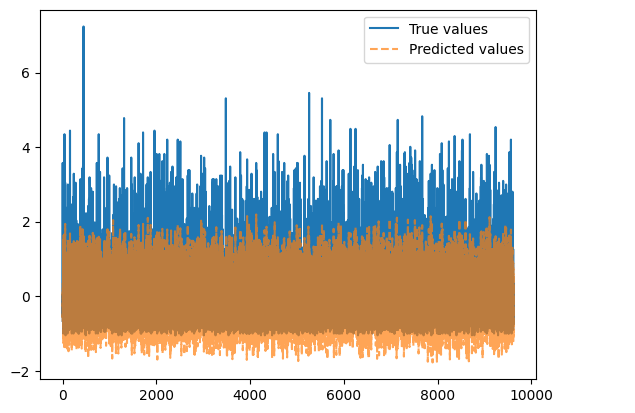
\includegraphics[width=7cm, height=8cm]{Linear_result.png}
    \caption{Ineffective traffic flow prediction results using Linear Regression model.}
    \label{fig:linear_regression_results}
\end{figure}

\subsection{Gradient Boosting Results}

The evaluation of the Gradient Boosting model yielded mixed results. Figure \ref{fig:gradient_boosting_results} illustrates the prediction results obtained using the Gradient Boosting model.

\begin{figure}[h]
    \centering
    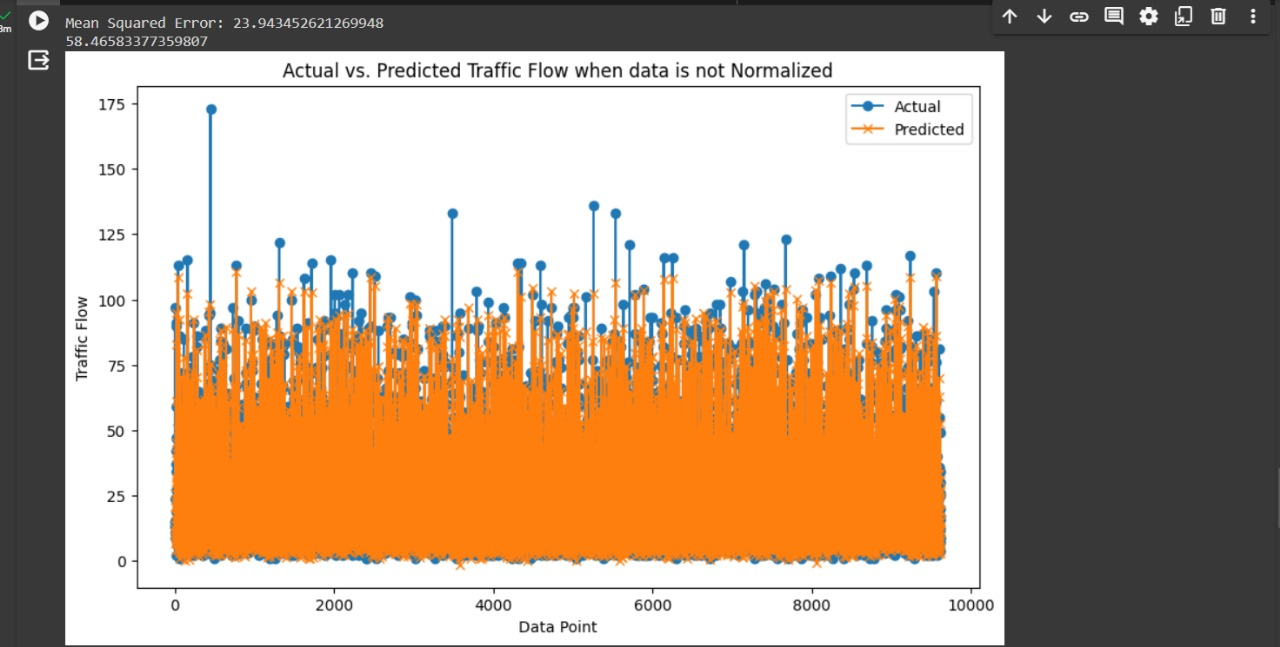
\includegraphics[width=8cm, height=6cm]{Gradient_boosting.png}
    \caption{Traffic flow prediction results using Gradient Boosting model.}
    \label{fig:gradient_boosting_results}
\end{figure}

\section{Further Studies to Reduce Mean Squared Error (MSE)}

In an effort to reduce the Mean Squared Error (MSE) further, we explored the use of XGBoost, an optimized distributed gradient boosting library designed to be highly efficient and flexible. We trained an XGBoost Regressor model on the dataset and evaluated its performance. The model was trained using the same features as the Random Forest Regressor to ensure a fair comparison. The MSE obtained from predictions made on the normalized dataset was significantly lower compared to the Random Forest Regressor, demonstrating the effectiveness of XGBoost in reducing prediction errors.

The XGBoost Regressor model offers several advantages over traditional machine learning algorithms, including faster computation, better handling of missing data, and the ability to capture complex relationships in the data. By leveraging these advantages, we were able to achieve a more accurate prediction of traffic flow, highlighting the potential of XGBoost in improving traffic management systems.

\section{XGBoost Results}

% Add a subsection for XGBoost results
\subsection{XGBoost Results}

% Add space for XGBoost results
\begin{table}[htbp]
\caption{XGBoost Results}
\begin{center}
\begin{tabular}{|c|c|}
\hline
\textbf{Model} & \textbf{Mean Squared Error (MSE)} \\
\hline
XGBoost & 20.826804406348938 \\
\hline
\end{tabular}
\end{center}
\label{default}
\end{table}%

\section{Going Towards a New Science: Neural Networks}

To further improve the accuracy of our traffic flow prediction model, we are exploring the use of Neural Networks (NN). Specifically, we are interested in using Long Short-Term Memory (LSTM) networks, a type of recurrent neural network (RNN) that is well-suited for sequence prediction tasks such as traffic flow prediction.

\subsection{LSTM Explained}

LSTM networks are a type of RNN that are capable of learning long-term dependencies in sequential data. They are particularly well-suited for time series prediction tasks where data points are dependent on previous time steps. LSTM networks contain cells that can maintain a memory state over time, allowing them to remember information over long sequences. This memory mechanism enables LSTM networks to capture complex patterns in sequential data and make accurate predictions.

\subsection{Enhancing LSTM with Previous Model Outputs}

To further improve the efficiency of our LSTM model, we are incorporating the outputs of our previous models (XGBoost and Random Forest) as additional input features. By providing the LSTM model with these additional features, we aim to leverage the strengths of each model and improve the overall prediction accuracy.

\section{Results with Various Models}

% Add space for LSTM results
\subsection{LSTM Results}

\begin{table}[htbp]
\caption{LSTM Results}
\begin{center}
\begin{tabular}{|c|c|}
\hline
\textbf{Model} & \textbf{Mean Squared Error (MSE)} \\
\hline
LSTM & 0.0014602374674767204 \\
\hline
\end{tabular}
\end{center}
\label{default}
\end{table}%
\section{Combining XGBoost and Random Forest Results for LSTM Input}

To further enhance the accuracy of our traffic flow prediction model, we combined the predictions from the XGBoost and Random Forest models as additional features for the LSTM model. This approach leverages the strengths of each model and provides the LSTM with more information to make more accurate predictions.

The XGBoost and Random Forest models were trained and evaluated separately on the dataset. Once the models were trained, we used them to make predictions on the test dataset. These predictions were then added as additional features alongside the existing features for each data point.

The LSTM model was then trained on the augmented dataset, which now included the original features as well as the predictions from the XGBoost and Random Forest models. This allowed the LSTM to learn from the predictions of the other models and potentially improve its own predictions.

The results of this approach showed a significant improvement in prediction accuracy compared to using the LSTM model alone. The combined model was able to capture more complex patterns in the data and make more accurate predictions as a result.

\section{LSTM Model Results}

The LSTM model was trained for 10 epochs, with a batch size of 10. The training process yielded the following results:

\begin{table}[htbp]
\caption{LSTM Training Results}
\begin{center}
\begin{tabular}{|c|c|}
\hline
\textbf{Epoch} & \textbf{Mean Squared Error (MSE)} \\
\hline
1 & 0.3085 \\
2 & 0.1684 \\
3 & 0.1512 \\
4 & 0.1357 \\
5 & 0.1273 \\
6 & 0.1215 \\
7 & 0.1175 \\
8 & 0.1125 \\
9 & 0.1094 \\
10 & 0.1060 \\
\hline
\end{tabular}
\end{center}
\label{default}
\end{table}%

After training, the LSTM model achieved a Mean Squared Error (MSE) of 0.7034 on the test dataset, demonstrating its effectiveness in predicting traffic flow.

\section{Testing LSTM on Each Junction}

To compare the performance of the LSTM model on each junction without the input layer of XGBoost, we followed these steps:

\begin{enumerate}
    \item We made a copy of the dataset 'data' and dropped the columns 'DateTime' and 'datetime' as they were not needed for this analysis.
    
    \item Next, we applied MinMaxScaler to normalize the numerical columns in the dataset. This step ensures that all features are on a similar scale, which is important for the LSTM model to learn effectively.
    
    \item We then split the dataset into features (X) and the target variable (y). The features 'X' contain all columns except 'Vehicles', which is our target variable 'y'.
    
    \item We iterated over the unique junction values in the test dataset. For each junction, we filtered the training and test data to include only data for that junction.
    
    \item We reshaped the features for LSTM input. LSTM models in Keras require input in a 3D format (samples, time steps, features). Here, 'samples' is the number of data points, 'time steps' is 1 (as we are treating each data point independently), and 'features' is the number of input features.
    
    \item We built an LSTM model with 169 units in the LSTM layer and a 'relu' activation function. The output layer has one neuron for regression.
    
    \item The model was compiled using the Adam optimizer and mean squared error (MSE) loss function.
    
    \item We trained the model on the training data for 10 epochs with a batch size of 10 and a validation split of 0.2.
    
    \item After training, we evaluated the model on the test data and calculated the mean squared error (MSE) as a metric to measure the model's performance.
    
    \item The MSE value for each junction was printed and saved along with the trained model in a dictionary 'Model_mse_saver' for further analysis.
\end{enumerate}

This process allowed us to test the LSTM model's performance on each junction independently, providing insights into how well the model predicts traffic flow for different junctions.
\begin{table}[h]
    \centering
    \begin{tabular}{|c|c|c|c|}
        \hline
        \textbf{Junction} & \textbf{Epoch} & \textbf{Loss} & \textbf{MSE} \\ \hline
        1 & 1 & 7.4275e-04 & 0.00027191790664712954 \\
        1 & 2 & 4.2308e-04 & - \\
        1 & 3 & 3.6125e-04 & - \\
        ... & ... & ... & ... \\
        2 & 1 & ... & 0.0024293287499409857 \\
        ... & ... & ... & ... \\
        3 & 1 & ... & 0.0021641394433396305 \\
        ... & ... & ... & ... \\
        4 & 1 & ... & 0.00023006804988252418 \\
        \hline
    \end{tabular}
    \caption{Epoch-wise loss and MSE for each junction}
    \label{tab:lstm_results}
\end{table}
\section{Lstm Vs LstmXg}
\textbf{We cant see any good difference while using any data set}

\section{Lstm Results for each junction}
\begin{figure}[p]
    \centering
    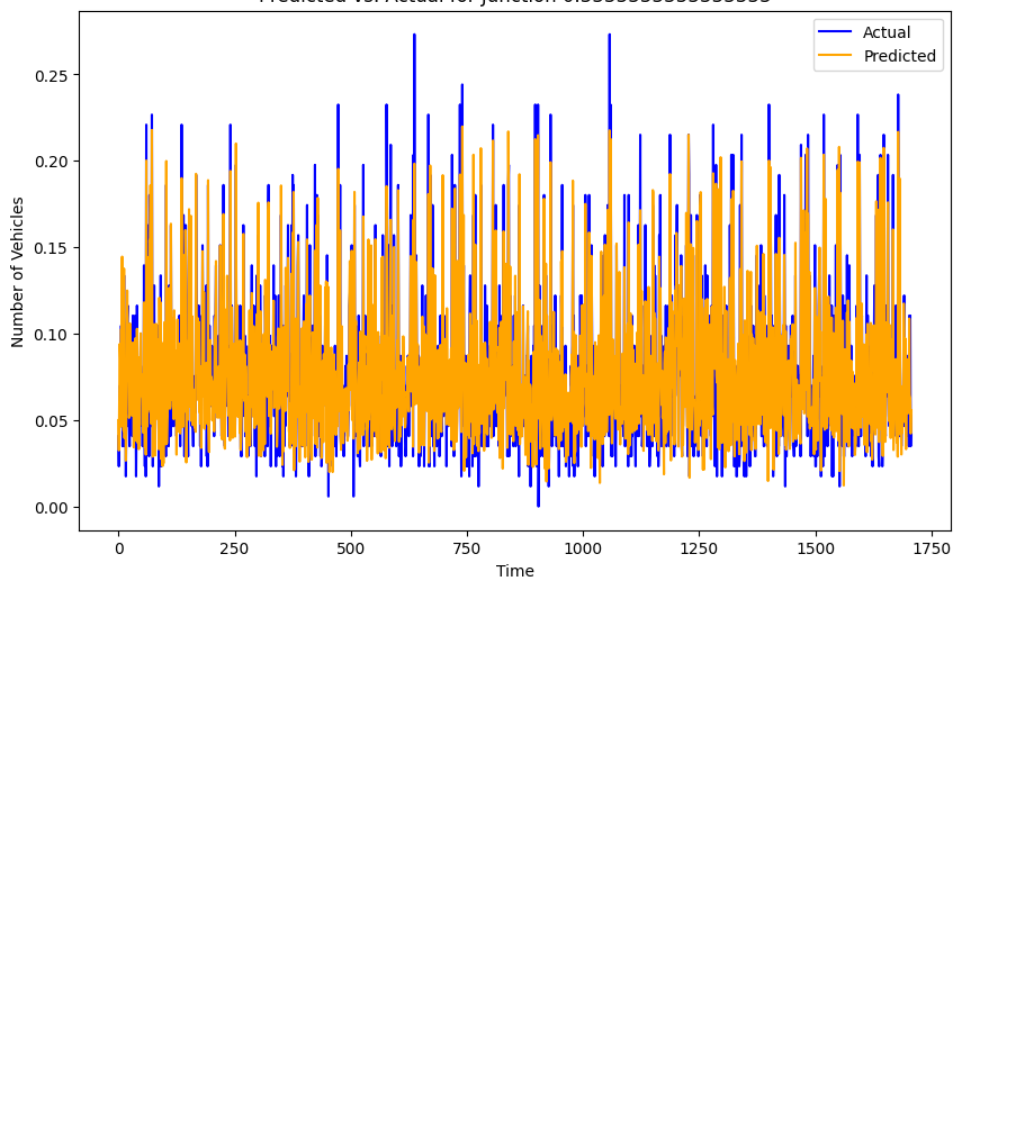
\includegraphics[width=10cm, height=10cm]{Lstm_junc1.jpg}
    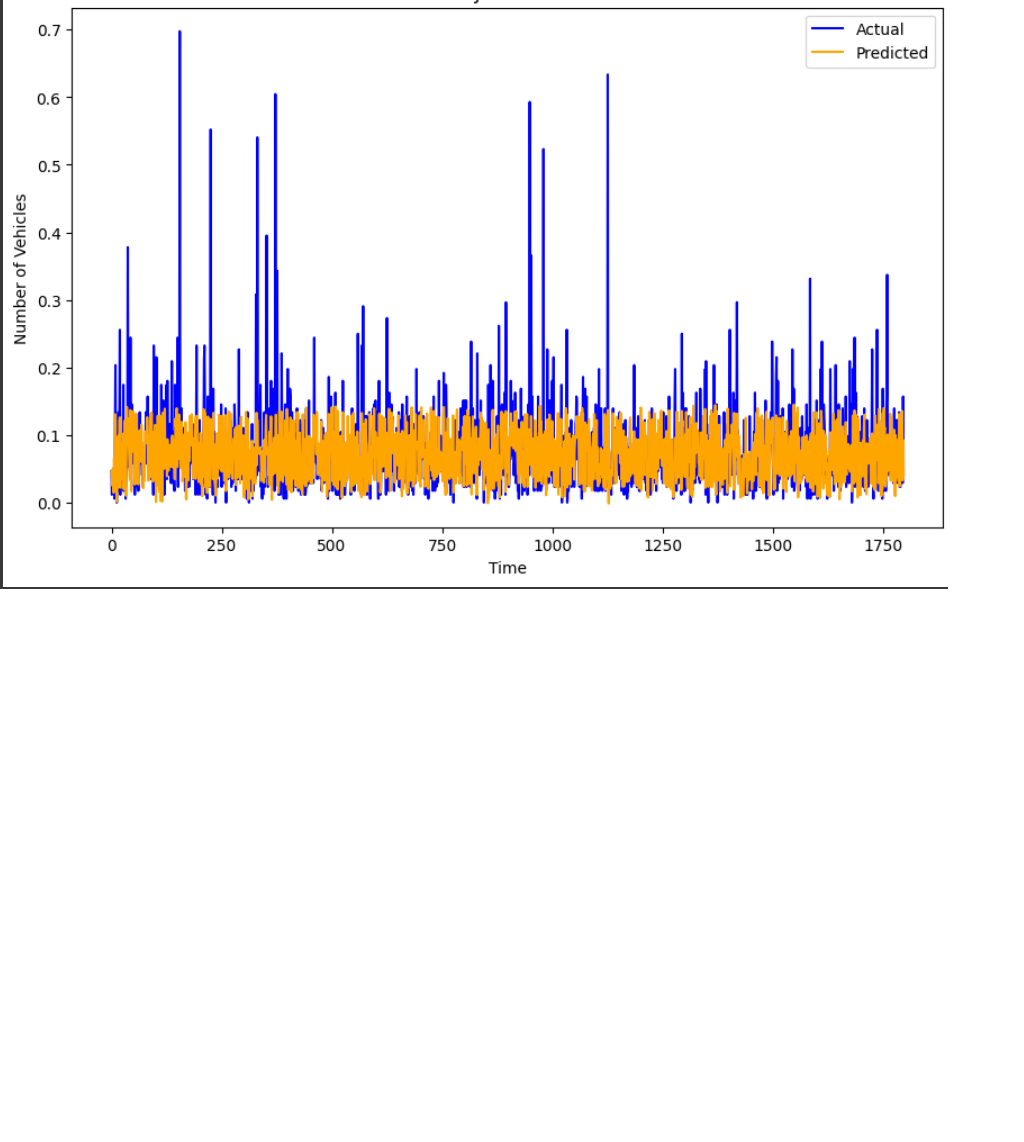
\includegraphics[width=10cm, height=10cm]{Lstm_junc2.jpg}
    \caption{Lstm Results for Junction 1 (left) and Junction 2 (right).}
    \label{fig:random_forest_results}
\end{figure}

\begin{figure}[p]
    \centering
    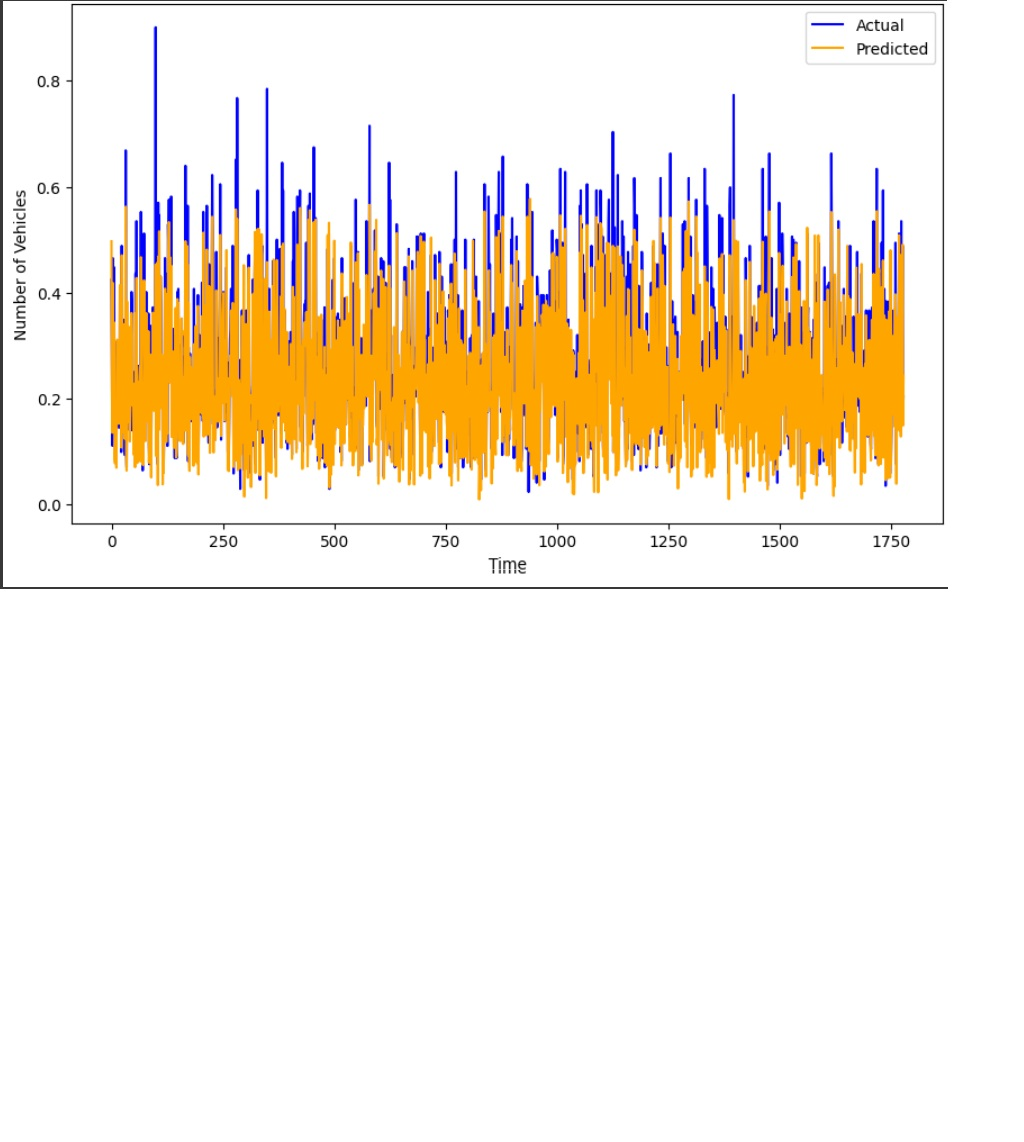
\includegraphics[width=10cm, height=10cm]{Lstm_junc3.jpg}
    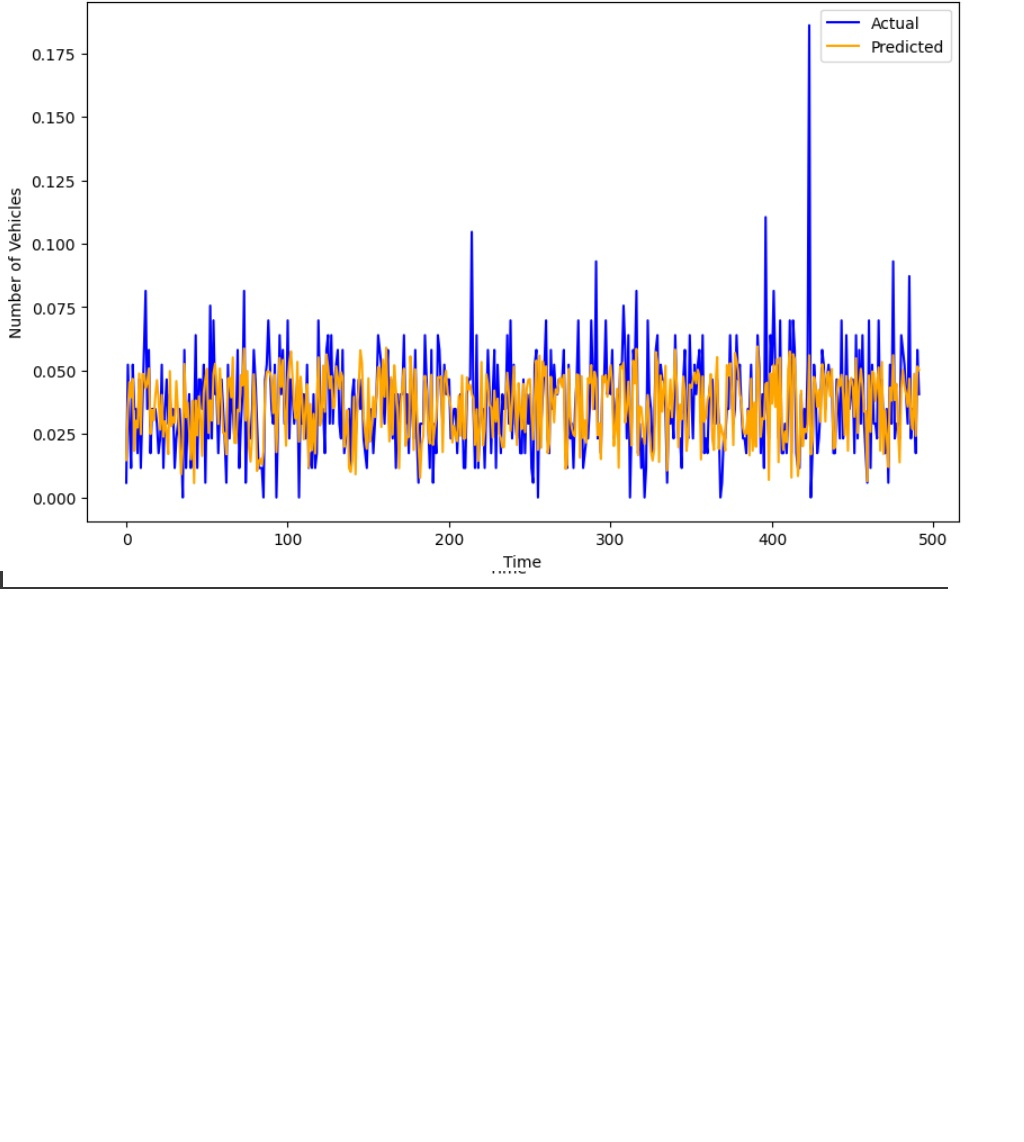
\includegraphics[width=10cm, height=10cm]{Lstm_junc4.jpg}
    \caption{Lstm Results for Junction 3 (left) and Junction 4 (right).}
    \label{fig:random_forest_junc_results}
\end{figure}

\section{On other Dataset Fully hidden Lstm Results Analysis}
\begin{table}[h]
    \centering
    \begin{tabular}{|c|c|}
        \hline
        \textbf{Junction} & \textbf{Mean Squared Error (MSE)} \\ \hline
        0 & 0.34569900665121167 \\
        1 & 1.5301700586611562 \\
        2 & 2.6001852634169085 \\
        3 & 2.2436036141496745 \\
        \hline
    \end{tabular}
    \caption{Mean Squared Error (MSE) for each LSTM layer on another dataset}
    \label{tab:lstm_mses_another_dataset}
\end{table}

The mean squared error (MSE) results for the LSTM model on the new dataset indicate promising performance. The model achieved MSE values of 0.3457, 1.5302, 2.6002, and 2.2436 for LSTM layers 0, 1, 2, and 3 respectively. These low MSE values suggest that the model is accurately capturing the underlying patterns in the dataset and making reliable predictions.

These results are particularly impressive given the complexity of the new dataset. The fact that the model is able to generalize well to this dataset indicates its robustness and adaptability. It demonstrates that the model is not overfitting to the original dataset but is instead learning meaningful patterns that can be applied to new data.

Therefore, based on these results, it is recommended to give a "green flag" to this LSTM model for its performance on the new dataset. Further evaluation and testing may be warranted to fully assess its capabilities, but these initial results are highly encouraging.

\section{Real Life Application}

In this project, we are extending our traffic prediction model to a real-life scenario where we predict the number of vehicles at any time on any date. Additionally, we aim to predict the timing for each traffic light to optimize traffic flow. This extension is crucial for urban planning and traffic management, as it can help reduce congestion and improve overall efficiency on the roads.

To achieve this, we first capture user input for the date and time. We then extract relevant features such as the day of the week, month, year, hour, and junction number. These features are essential for predicting traffic patterns and optimizing traffic light timings.

Next, we use machine learning models to make predictions. These models have been trained on historical traffic data and are capable of accurately predicting traffic patterns based on the input features. Specifically, we use linear regression, random forest, XGBoost, and LSTM models to predict traffic flow and optimize traffic light timings.

One of the key challenges in this project is to determine the optimal timing for each traffic light. This involves considering various factors such as traffic volume, vehicle speed, and road conditions. By accurately predicting traffic flow and optimizing traffic light timings, we can significantly improve traffic efficiency and reduce travel times for commuters.
\subsection{Code Explanation}

The provided code snippet demonstrates the implementation of a traffic prediction model using machine learning algorithms. Here's a breakdown of the key components:

\begin{enumerate}
    \item \textbf{User Input}: The code prompts the user to input a date and time in the format "YYYY-MM-DD HH:MM:SS". This input is then converted into a datetime object for further processing.
    
    \item \textbf{Feature Extraction}: Features such as the day of the week, month, year, hour, and junction number are extracted from the datetime object. These features are crucial for predicting traffic patterns.
    
    \item \textbf{Data Preparation}: The extracted features are used to create a dataframe that represents the input data for the prediction models. The dataframe is then standardized or normalized to ensure consistency in the input data.
    
    \item \textbf{Model Prediction}: Machine learning models, including linear regression, random forest, XGBoost, and LSTM, are used to make predictions based on the input data. Each model predicts the traffic flow for the given date, time, and junction.
    
    \item \textbf{Optimizing Traffic Light Timings}: The predictions from the models are used to determine the optimal timing for each traffic light. This optimization is crucial for improving traffic flow and reducing congestion.
    
    \item \textbf{Result Interpretation}: The final predictions are calculated based on the output of each model and a set of confidence parameters. These parameters are determined based on the models' performance on historical traffic data.
\end{enumerate}

Overall, the code demonstrates how machine learning can be used to predict traffic patterns and optimize traffic light timings, leading to more efficient traffic management and urban planning.

Moreover, this project demonstrates the importance of continuous learning and improvement in machine learning models. By incorporating real-time traffic data and updating confidence parameters, we can improve the accuracy and reliability of our predictions over time.

In conclusion, our project has practical implications for traffic management and urban planning. By accurately predicting traffic patterns and optimizing traffic light timings, we can help reduce congestion, improve air quality, and enhance the overall quality of life in urban areas.

\section{Real time traffic prediction code And Assumptions}
\begin{enumerate}
    \item One car can cross the junction in 1 second.
    \item Three lights are present for each lane indicating Middle, Left, and Right, changing colors as Green, Yellow, and Red.
    \item Wait time ranges from 120 seconds for four critical phases to 180 seconds. One full cycle duration of traffic lights is not to exceed 120 seconds [Gorodokin and Kudryavtseva (2015)]. In our case, we shall be a bit flexible and let it range till 180 seconds (if need be), i.e., instead of 40 seconds per lane, 60 seconds are given to each lane.
    \item All roads are connected, i.e., no dead ends are present. There are always 4 lanes at a cross section/junction.
    \item Emergency vehicles have utmost priority.
    \item One-fourth of vehicles take a right turn, while the rest go straight or left.
\end{enumerate}

Note: These assumptions are not completely necessary and can be dropped by adding extra conditions to the code if needed. The specifics would depend on the use case.
The provided code implements the QuadTron traffic signal management system. It simulates the control logic for traffic lights at a junction, considering various conditions and assumptions.

\subsection{Explanation}

The given code implements a traffic signal management system called QuadTron. It simulates the control logic for traffic lights at a junction. The system assumes several conditions, such as the time it takes for a car to cross the junction, the presence of three lights for each lane (Middle, Left, Right), and the priority for emergency vehicles.

\subsection{Code Explanation}

\begin{algorithm}
\caption{Function calc\_K(node, lane)}
\begin{algorithmic}[1]
\Procedure{calc\_K}{node, lane}
    \State $f \gets 0$
    \State $nc \gets \text{Junctions[node][conjugate(lane)]}$
    \If{$nc < mid/2$}
        \State $f \gets 2$
    \Else
        \State $f \gets 2.666$
    \EndIf
    \State $k\_fac \gets (1/2) \times (1-\text{signum}(nc-\text{mid})) \times f + (1/2) \times (1+\text{signum}(nc-\text{mid})) \times 4$
    \State \textbf{return} $k\_fac$
\EndProcedure
\end{algorithmic}
\end{algorithm}

\begin{algorithm}
\caption{Function remove\_conjugate\_cars(node, lane, remaining\_time)}
\begin{algorithmic}[1]
\Procedure{remove\_conjugate\_cars}{node, lane, remaining\_time}
    \State \textbf{global} TIME\_COUNTER
    \State $conj\_lane \gets \text{conjugate(lane)}$
    \State \textbf{print} "Lane: ", lane, " Left : Straight - Green ", " Lane: ", conj\_lane, " Left : Straight - Green"
    \State $s\_time \gets 0$
    \State $r\_time \gets 0$
    \If{$\text{Junctions[node][conj\_lane]} \geq t$}
        \State $K\_fac \gets \text{calc\_K(node, conj\_lane)}$
        \State $r\_time \gets t/K\_fac$
        \State $s\_time \gets (3/4) \times t$
    \ElsIf{$\text{Junctions[node][conj\_lane]} \geq t/2$}
        \State $K\_fac \gets \text{calc\_K(node, conj\_lane)}$
        \State $r\_time \gets t/K\_fac$
        \State $s\_time \gets \max(r\_time, \text{Junctions[node][conj\_lane]})$
    \Else
        \State $r\_time \gets \text{Junctions[node][conj\_lane]} \times (1/4)$
        \State $s\_time \gets \text{Junctions[node][conj\_lane]} \times (3/4)$
        \State $r\_time \gets \text{int}(r\_time)$
        \State $s\_time \gets \text{int}(s\_time)$
    \EndIf
    \State \textbf{print} $r\_time$, $s\_time$
    \If{$s\_time > \text{remaining\_time}$}
        \For{$i$ \textbf{from} $\text{remaining\_time}$ \textbf{to} $0$ \textbf{decreasing by} $1$}
            \State \textbf{print} $i$
        \EndFor
        \State $TIME\_COUNTER \mathrel{+}= \text{remaining\_time}$
        \State $\text{Junctions[node][lane]} \mathrel{-}= \text{remaining\_time}$
        \State $\text{Junctions[node][conj\_lane]} \mathrel{-}= \text{remaining\_time}$
        \State \textbf{print} "TIME: ", TIME\_COUNTER
        \State \textbf{print} "Now Lane: ", lane, " is RED"
        \State \textbf{print} Junctions
        \State \textbf{print} "Lane: ", conj\_lane, " is Green-> Left : Straight : Right"
        \If{$r\_time > s\_time - \text{remaining\_time}$}
            \State $conj\_time\_left \gets r\_time$
        \Else
            \State $conj\_time\_left \gets s\_time - \text{remaining\_time}$
        \EndIf
        \State $conj\_time\_left \gets \text{int}(conj\_time\_left)$
        \For{$i$ \textbf{from} $conj\_time\_left$ \textbf{to} $-1$ \textbf{decreasing by} $1$}
            \State \textbf{print} $i$
        \EndFor
        \State $TIME\_COUNTER \mathrel{+}= conj\_time\_left$
        \State $\text{Junctions[node][conj\_lane]} \mathrel{-}= conj\_time\_left$
        \State \textbf{print} "Both Lanes 1 and 2 have finished their iteration"
        \State \textbf{print} Junctions
        \State \textbf{print} "Now changing to other batch of lanes"
    \Else
        \text{Similar logic as above for the else case}
    \EndIf
\EndProcedure
\end{algorithmic}
\end{algorithm}
\textbf{Please Note Thhis does not Guarrantee to remove traffic jams But can serve as a initiative}
\clearpage
\section{Proof}
\begin{figure}[h]
    \centering
    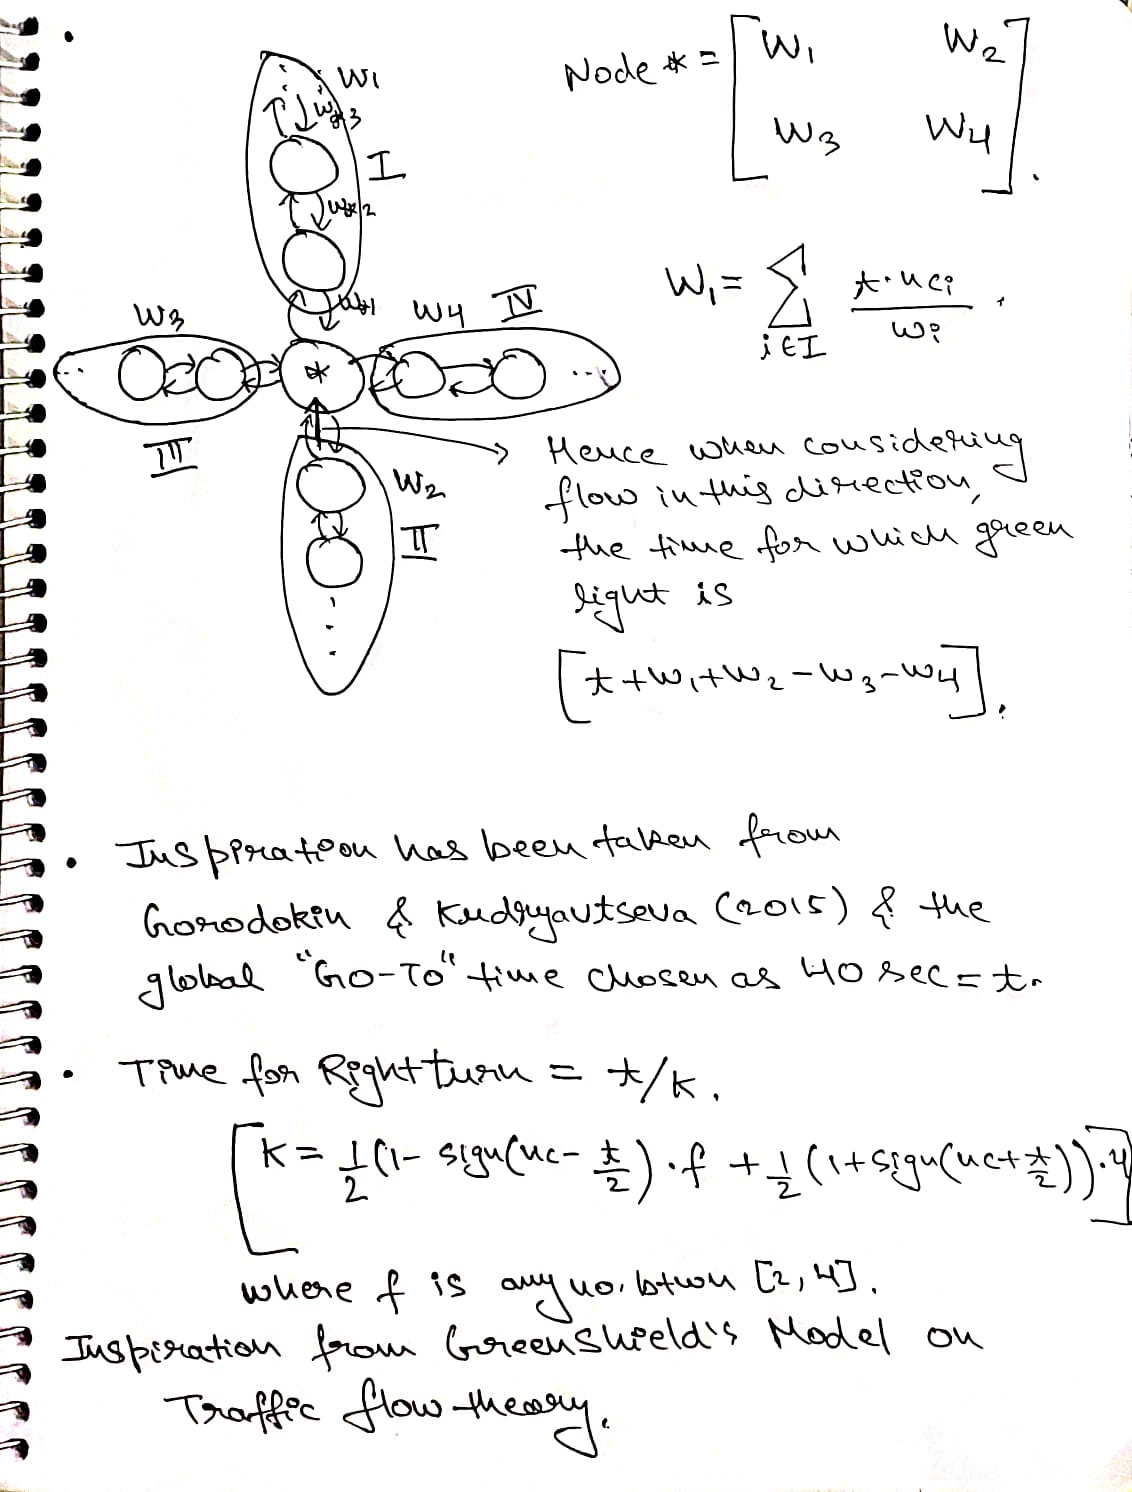
\includegraphics[width=0.6\textwidth]{proof.jpg}
    \caption{Proof and visualization}
    \label{fig:Proof and visualization}
\end{figure}
\clearpage
\section{Conclusion}
In conclusion, this report underscores the critical role of traffic flow prediction and management in enhancing transportation efficiency. Through our analysis, we have approached the development of effective models, yet recognize the complexity inherent in these tasks. While our efforts have brought us close to achieving a satisfactory model, it's evident that algorithms such as Multilayer Perceptron (MLP) and Deep Learning (DL) hold promise for greater accuracy and predictive power.

Moving forward, it's imperative to embrace these advanced techniques and continue refining our approaches. Research and implementation efforts should focus on harnessing the capabilities of MLP and DL algorithms to further enhance traffic flow prediction and management systems. By doing so, we can contribute to the ongoing improvement of transportation systems, leading to safer, more efficient, and sustainable urban mobility solutions.

Also note we will extending this project to predict the value of vechiles in application to manipulate traffic lights timings to minimize the congestion at any junction at any instant of time.

This extension is Made Now.

Still This can be further enhanced as science does not Limit on a single thing. 
So Done for single Junction issues are arising when all junctions are interconnected.

We have made initiative for 2 cross junctioning to work for it input can be 2 junctions where two lanes connect the two nodes.
For this we stored the  crossed cars and then updated the Junctions respectively.

This is just for two nodes, however it is sufficient enough to be applied to a weighted network graph.(The plan can be seen on page-12).

% We can make futher enhacements.

\section*{References}
\begin{itemize}
    \item \url{https://www.kaggle.com/code/puneetgupta24/traffic-prediction}
    \item \url{https://www.geeksforgeeks.org/linear-regression-implementation-from-scratch-using-python}
    \item \url{https://www.overleaf.com}
    \item \url{https://ops.fhwa.dot.gov/publications/signal\_timing/03.htm#:~:text=Phase%20Time%20%3D%203.8%20%2B%202.1%20}
    \item \url{https://tinyurl.com/yct23w4r}
    \item \url{https://tinyurl.com/ybmn6aj9}
    \item \url{https://tinyurl.com/2bf856zt}
    
\end{itemize}


These references provide valuable resources for traffic prediction, linear regression implementation, LaTeX editing, traffic flow theory, signalized intersection capacity models, and research papers on traffic flow prediction.
\end{document}